\documentclass[bachelor,german]{hgbthesis}
% Zulässige Class Options: 
%   Typ der Arbeit: diplom, master (default), bachelor, praktikum 
%   Hauptsprache: german (default), english
%%------------------------------------------------------------
\graphicspath{{images/}}    % name of directory containing the images
\logofile{FHOOeIntl2014}			% name of PDF, remove or use \logofile{} for no logo
\AddBibFile{literatur}  	% name of the BibTeX (.bib) file


%%%----------------------------------------------------------
\begin{document}
%%%----------------------------------------------------------

% Einträge für ALLE Arbeiten: --------------------------------
\title{Konzeption eines Mail Service}
\author{Ing. Thomas Herzog}
\studiengang{Software Engineering}
\studienort{Hagenberg}
\abgabedatum{2016}{02}{01}	% {YYYY}{MM}{DD}
%%% zusätzlich für eine Bachelorarbeit: ---------------------
\nummer{S1310307011-A}   % XX...X = Stud-ID, z.B. 0310238045-A  
                        % (A = 1. Bachelorarbeit)
\semester{Wintersemester 2015/16} 
\gegenstand{Software Engineering} 
\betreuer{FH-Prof. DI Dr. Heinz Dobler} % oder \betreuerin{..}
%\strictlicense  % erzeugt restriktive Lizenzformel

%%%----------------------------------------------------------
\frontmatter
\maketitle
\tableofcontents
%%%----------------------------------------------------------

\chapter{Vorwort} 	% engl. Preface
Folgende Arbeit beschäftigt sich mit der Konzeption einer Mail-Anwendung für die Firma curecomp GembH, welche in weiterer Folge als \emph{CleverMail}\newline
bezeichnet wird, die eine bestehende Mail-Anwendung, in weiterer Folge\newline
\emph{CCMail} genannt, ablösen soll. Die  Firma curecomp GembH ist ein Dienstleister im Supplier Relationship Management (SRM) und betreibt eine Softwarelösung, die aus zwei Anwendungen besteht:\newline
\begin{enumerate}
	\item\emph{CleverWeb}\newline
	Eine Web-Anwendung für den webbasierten Zugriff
	\item\emph{CleverInterface}\newline
	Eine Schnittstellen-Anwendung für die Anbindung der ERP-Systeme der Kunden und Lieferanten
\end{enumerate} 
\ \newline
Beide Anwendungen erfordern den Versand von E-Mail-Nachrichten um verschiedene Systemzustände den Benutzern mitzuteilen wie z.B.:
\begin{itemize}
	\item Fehlermeldungen
	\item Statusänderungen bei Bestellungen (erstellt, geliefert, storniert, ...)
	\item Lieferverzugsmeldungen
	\item ...
\end{itemize}
\ \newline
Es wurden neue Anforderungen für \emph{CCMail}
definiert, die sich nicht mehr in \emph{CCMail} integrieren lassen. Dies ist begründet in dem Design und der Implementierung von \emph{CCMail}.
\newline\newline
Diese Arbeit wird sich einerseits mit der Diskussion des bestehenden Designs und der bestehenden Implementierung von \emph{CCMail} befassen und andererseits ein Konzept für 
\emph{CleverMail} einbringen. Das eingebrachte Konzept soll als Basis für die praktische Bachelorarbeit dienen, in der das eingebrachte Konzept umgesetzt werden soll.
		% ggfs. weglassen
\chapter{Kurzfassung}
Die vorliegende Bachelorarbeit behandelt das Vorlagenmanagement für die Anwendung \emph{CleverMail}, die in der theoretischen Bachelorarbeit konzipiert wurde und eine Anwendung ist, die zum Versand von \emph{E-Mails} verwendet wird. Mit dem Vorlagenmanagement können Vorlagen für die \emph{E-Mail}-Nachrichten zur Laufzeit und in mehreren Sprachen verwaltet werden.
\newline
\newline
Das Vorlagenmanagement verwendet mehrere Technologien und Sprachen wie \emph{CDI}, \emph{JSF} und \emph{TypeScript}. Vor allem die Implementierung in Java 8 und die Möglichkeit der Verwendung der neuen sprachspezifischen Funktionalitäten wie \emph{Lambda}-Ausdrücke, Methodenreferenzen und die \emph{Stream-API} haben den Quelltext vereinfacht.
\newline
\newline
Die Integration des Vorlagenmanagements in eine \emph{CDI}-Umgebung war einfach zu realisieren und hat gezeigt, dass ein Softwaremodul in eine \emph{CDI}-Umgebung einfach integriert werden kann, sofern es die nötigen Voraussetzungen erfüllt. Die implementierte \emph{CDI}-Erweiterung wird einfach zu erweitern sein und man könnte mehr Funktionalitäten, die in \emph{CDI} zur Verfügung stehen, verwenden. Es könnten z.B. Erzeuger für Variablen registriert werden, die zur Laufzeit dynamisch Variablen erzeugen, anstatt die Variablen nur beim Start der \emph{CDI}-Umgebung zu registrieren, welche dann über die Lebensdauer der \emph{CDI}-Umgebung  unveränderlich sind. 
\newline
\newline
Während der Entwicklung des Vorlagenmanagements sind keine erwähnenswerten Probleme aufgetreten, alle Funktionalitäten und die Integration konnten einfach implementiert und getestet werden, wobei besonders die Einfachheit der Tests in einer \emph{CDI}-Umgebung hervorgehoben werden muss, die mit der verwendeten Bibliothek \emph{DeltaSpike} einfach aufgesetzt werden können und innerhalb einer Entwicklungsumgebung, ohne Anwendungsserver, lauffähig sind.
\newline
\newline
Die Implementierung des \emph{CKEditor-Plugins} gestaltete sich einfach, da dieser \emph{Editor} gut dokumentiert ist und es bereits Typinformationen für \emph{TypeScript} gibt. Der \emph{Editor TinyMCE}, für den anfangs das \emph{Plugin} entwickelt werden sollte, ist hingegen schlecht dokumentiert, daher wurde auf den \emph{Editor CKEditor} gewechselt. Die Implementierung in \emph{TypeScript} war die richtige Entscheidung, denn es hat die Entwicklung vereinfacht, und der Quelltext ist lesbarer als der Quelltext in \emph{JavaScript}. Für die Zukunft wird \emph{TypeScript} weitere sprachspezifische Möglichkeiten bieten, die den Quelltext noch mehr vereinfachen werden, obwohl eine Migration auf eine neuere Version von \emph{TypeScript} zur Zeit nicht nötig ist.		
\chapter{Abstract}

TODO: Add english summary here
			

%%%----------------------------------------------------------
\mainmatter         % Hauptteil (ab hier arab. Seitenzahlen)
%%%----------------------------------------------------------

\chapter{Einleitung}
\label{cha:Einleitung}
Die vorliegende Sachlage beschäftigt sich mit der Konzeption und Implementierung eines Vorlagen-\emph{Management} für den in der theoretischen Bachelorarbeit konzipierten \emph{Mail}-Service. Das Vorlagen-\emph{Management} stellt einen essentiellen Teil des \emph{Mail}-Service dar, mit dem sich parametrisierte \emph{E-Mail}-Vorlagen erstellen lassen. Das Vorlagen-\emph{Management} soll es den BenutzerInnen ermöglichen einfach eigene parametrisierte \emph{E-Mail}-Vorlagen zu erstellen, die in einer Anwendung, die den \emph{Mail}-Service nutzen, verwendet werden können, um benutzerspezifische \emph{E-Mail}-Nachrichten zu versenden. Mit dem Vorlagen-\emph{Management} ist es nicht mehr erforderlich die \emph{E-Mail}-Vorlagen statisch zu definieren und die \emph{E-Mail}-Vorlagen können von den Benutzerinnen nach ihren Wünschen angepasst werden.  

\section{Das Unternehmen curecomp Software Service GmbH}
Diese Arbeit wird in Zusammenarbeit mit dem Unternehmen \emph{curecomp Software Service GembH} erstellt. Das Unternehmen \emph{curecomp} ist ein ein Dienstleister im \emph{Supplier-Relationship-Management (SRM)} und betreibt eine eigene Softwarelösung namens \emph{clevercure}. Die Softwarelösung \emph{clevercure} besteht aus den folgenden Anwendungen:
\begin{itemize}
	\item\emph{CleverWeb} ist eine \emph{Web}-Anwendung für den webbasierten Zugriff auf \emph{clevercure}.
	\item\emph{CleverInterface} ist eine Schnittstellen-Anwendung für den XML-basierten Datenimport /-export zwischen clevercure und den ERP-Systemen der Kunden.
	\item\emph{CleverSupport} ist eine unternehmensinterne \emph{Web}-Anwendung für die Abwicklung von \emph{Support}-Prozessen.
	\item\emph{CleverDocument} ist ein Dokumentenmanagementsystem für die Verwaltung aller anfallender Dokumente innerhalb von \emph{clevercure}.
	\item\emph{CCMail} ist die bestehende \emph{Mail}-Anwendung für den Versand aller innerhalb \emph{clevercure} anfallender \emph{E-Mail}-Nachrichten.
\end{itemize}
\ \newline
Wie bereits in der theoretischen Bachelorarbeit behandelt, wird \emph{CCMail} von \emph{CleverMail} abgelöst werden, wobei dass in dieser Arbeit behandelte Vorlagenmanagement die Grundlage für \emph{CleverMail} darstellt. Alle Anwendung innerhalb der Softwarelösung \emph{clevercure} haben die Anforderung das \emph{E-Mail}-Vorlagen parametrisiert und benutzerdefiniert erstellt werden können. Diese Anforderung wird mit dem Vorlagenmanagement erfüllt.

\section{Das Vorlagenmanagement für den \emph{Mail}-Service}
Mit dem Vorlagenmanagement können \emph{E-Mail}-Vorlagen einerseits von den EntwicklerInnen und BenutzerInnen benutzerdefiniert und parametrisiert erstellt werden. Damit können \emph{E-Mail}-Vorlagen dynamisch auch zur Laufzeit erstellt, modifiziert und gelöscht werden. Es sind keine statischen \emph{E-Mail}-Vorlagen mehr nötig und alle damit verbunden Nachteile wie z.B. 
\begin{itemize}
	\item das neu Kompilieren und Einspielen bei Änderungen der \emph{E-Mail}-Vorlagen,
	\item keine Möglichkeit für benutzerdefinierten Vorlagen oder
	\item keine Möglichkeit der Nutzung von dynamischen Parametern in den \emph{E-Mail}-Vorlagen
\end{itemize}
\ \newline
eliminiert werden. Das Vorlagenmanagement kann auch in einem anderen Kontext verwendet werden, wobei diese Arbeit sich  ausschließlich mit der Verwendung des Vorlagenmanagement innerhalb des \emph{Mail}-Service beschäftigen wird. 
\newline
TODO: Add graphic about template management
\newline

\section{Die Rahmenbedingungen}
Das Vorlagenmanagement wird in Java in der Version 8 implementiert und wird sich an der \emph{Java-Enterprise-Edition 7 (JEE-7)} Spezifikation orientieren, wobei folgende Teilspezifikationen Anwendung finden.
\begin{itemize}
	\item \emph{JPA 2.1} ist die Spezifikation für die Persistenz.
	\item \emph{CDI 1.1} ist die Spezifikation für kontextabhängige Injektion innerhalb einer \emph{JEE7}-Umgebung.
	\item \emph{JSF 2.2} ist die Spezifikation der \emph{View}-Technologie. 
\end{itemize}
\ \newline
Damit wird das Vorlagenmanagement mit den aktuellsten Standards implementiert und wird daher für die Zukunft gut gewappnet sein. Die Funktionalität des Vorlagenmanagement wird weitestgehend ohne die Verwendung spezieller Bibliotheken implementiert, wobei folgende Integrationen zur Verfügung gestellt werden.
\begin{itemize}
	\item \emph{CDI}-Integration:
	\newline
	Innerhalb eines \emph{CDI-Containers} werden Objekte kontextabhängig zur Verfügung gestellt.
	\item \emph{JSF}-Integration:
	\newline
	Mit der \emph{View}-Technologie \emph{JSF} wird eine Webseite erstellt, über die die Vorlagen verwaltet werden können.
	\item \emph{Typescript}-Integration:
	\newline
	Mit \emph{Typescript} wird ein \emph{Plugin} für den \emph{Rich-Editor CKEditor} implementiert, welches die Variablen für eine \emph{E-Mail}-Vorlage innerhalb des \emph{CKEditors} verwaltet.
\end{itemize} 
\ \newline
Als Entwicklungsumgebung wird die \emph{IDE Intellij} verwendet, die eine bekannte Entwicklungsumgebung im \emph{Java}-Umfeld darstellt und ein Produkt des Unternehmens \emph{Jetbrains} mit Sitz in Tschechien ist. Als Applikationsserver wird \emph{Wildfly 10.x}, vormals \emph{JbossAS} genannt, des Unternehmens  \emph{Redhat} verwendet, der ein zertifizierter \emph{JEE-7}-Server ist und somit alle benötigten Spezifikationen unterstützt.

\chapter{Die alte Anwendung \emph{CCMail}}
\label{cha:ccmail}
In diesem Kapitel wird die alte Anwendung \emph{CCMail} analysiert und diskutiert. Ziel ist es, einen Überblick über diese Anwendung und deren wesentlichsten Aspekte zu liefern, sowie diese Aspekte genauer zu betrachten. Die Ergebnisse dieser Analyse sollen als Grundlage für das neue Konzept dienen, das auch die Integration in die bestehenden Anwendungen berücksichtigen muss. Diese Integration soll mit geringst möglichen Aufwand erfolgen können, da Probleme bei der Integration negative Auswirkungen auf den produktiven Betrieb haben könnten. 

\section{Systemaufbau}
\label{sec:ccmail-systemaufbau}
Im folgenden wird der Systemaufbau aus der Sicht der Anwendung \emph{CCMail} und dessen Integration in das System über \emph{MailJobs} diskutiert. 
\begin{figure}[h]
\centering
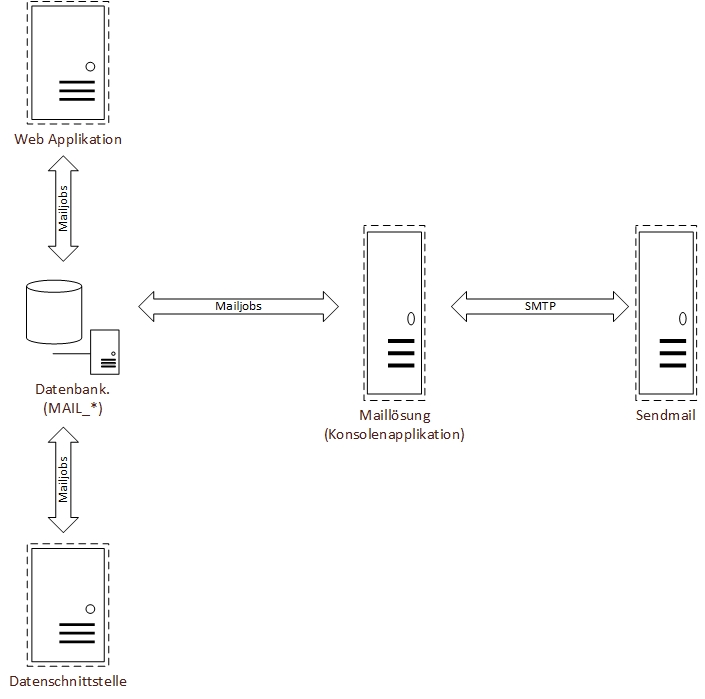
\includegraphics[scale=0.38]{Systemaufbau_alt.jpg} %{CS0031}
\caption{Systemaufbau und Integration von \emph{CCMail}}
\label{fig:ccmail-system-und-integration}
\end{figure}
\ \newpage
\parindent0pt{Abbildung} \ref{fig:ccmail-system-und-integration} zeigt das Gesamtsystem aus der Sicht der Anwendung \emph{CCMail}, wobei anzumerken ist, dass das System bis heute angewachsen ist und nunmehr aus mehreren Anwendungen als wie in Abbildung  \ref{fig:ccmail-system-und-integration} abgebildet besteht. Es lässt sich ableiten, dass das Kernstück des Systems die Datenbank ist. In der Datenbank werden die zu versendenden \emph{E-Mails}, als sogenannte \emph{MailJobs}, verwaltet. Ein \emph{MailJob} ist ein Eintrag in einer Datenbanktabelle namens \emph{MAIL\_JOBS}, die alle Informationen einer \emph{E-Mail} enthält. Es sind dabei die eigens implementierten Datenbankzugriffsschichten der einzelnen Anwendungen zu kritisieren, die zwar den Datenbankzugriff kapseln, jedoch nur für jede Anwendung an sich und nicht über Anwendungsgrenzen hinweg, was durchaus möglich wäre. Scott W.Ambler und Parmod J.Sadalge schreiben in ihrem Buch \cite[27]{refactoreDatabase} treffend:
\begin{quote}
\emph{The greater the coupeling, the harder is to refactore something. This is true of code refactoring, and it is certainly true of database refactoring}
\end{quote}
Da jede Anwendung ihre eigene Datenzugriffsschicht implementiert, muss jede Anwendung bei einer Datenbankänderung ihre Implementierung anpassen. Eine zentrale Datenbankzugriffsschicht würde nur eine Änderung an einer Stelle erfordern. Also haben wir hier eine Form der starken Koppelung die sich durch die Code-Duplikate ausprägt.
\newline
\newline
Die Anwendungen \emph{CleverWeb} und \emph{CleverInterface} erstellen über ihre eigens implementierten Datenbankzugriffsschichten \emph{MailJob-Entitäten} in der Datenbank, welche zeitgesteuert von \emph{CCMail} ausgelesen, verarbeitet und in Form von \emph{E-Mails} versendet werden. \emph{CCMail} ist als Konsolen-Anwendung implementiert und enthält alle Ressourcen, die es benötigt, um die \emph{MailJob-Entitäten} zu verarbeiten. Auch hier wirken sich die eigens implementierten Datenbankzugriffsschichten aus, da es keine einheitliche Spezifikation für das Erstellen eines \emph{MailJobs} gibt. Validierungen, ob ein zu erstellender \emph{MailJob} gültig ist, werden den einzelnen Anwendungen überlassen und sind nicht an einer zentralen Stelle umgesetzt. Daher muss sich die Implementierungen in \emph{CCMail} darauf verlassen, dass alle Anwendungen die \emph{MailJobs} korrekt anlegen, damit diese von \emph{CCMail} korrekt verarbeitet werden können.
\newline
\newline
Als Mail-Server wird \emph{Sendmail} verwendet. Es handelt sich hierbei um eine Anwendung, die für Linux Distributionen frei verfügbar ist. \emph{CCMail} versendet die \emph{E-Mails} über SMTP \emph{(Simple Mail Transport Protocol)} an \emph{Sendmail}, welches die \emph{E-Mails} seinerseits an die EmpfängerInnen versendet.

\newpage
\section{\emph{E-Mail}-Versand}
\label{sec:ccmail-email-versand}
Der im folgenden beschriebene Prozess des \emph{E-Mail}-Versands zeigt auf wie hinsichtlich des Systemaufbaus beschrieben in \ref{sec:ccmail-systemaufbau} der \emph{E-Mail}-Versand vom Anlegen eines \emph{MailJobs} bis hin zum Versand der eigentlichen \emph{E-Mail} funktioniert. 
\newline
\newline
Als Kernkomponente des Systems wurde die Datenbank identifiziert, welche die \emph{MailJob}-Entitäten hält, die wiederum von \emph{CCMail} aus der Datenbank gelesen und verarbeitet werden. Dieser Ansatz ist an sich nicht als schlecht anzusehen, jedoch verbirgt sich hier eines der Hauptprobleme des \emph{E-Mail}-Versands, nämlich die Inkonsistenz der versendeten \emph{E-Mail}, durch die Zeitdifferenz zwischen dem Anlegen eines \emph{MailJobs} durch die Anwendungen und dem tatsächlichen Versand der \emph{E-Mail} durch \emph{CCMail}.
\begin{figure}[h]
\centering
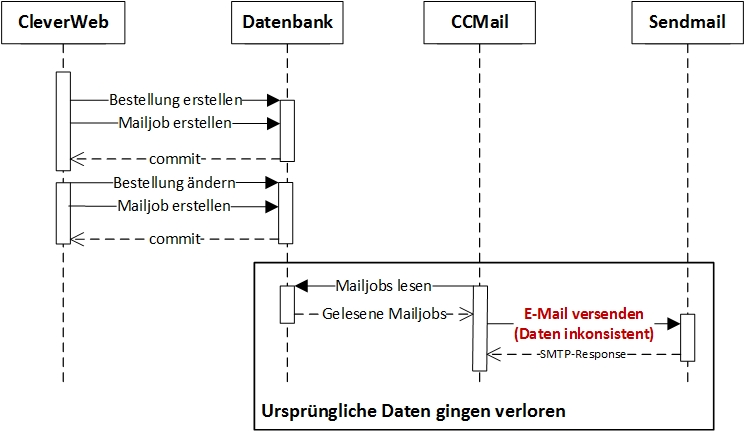
\includegraphics[scale=0.8]{prozess_sequence_emailversand.jpg}
\caption{Gesamtprozess des \emph{E-Mail}-Versands}
\label{fig:sequence-diagramm-gesamtprozess}
\end{figure}
\ \newline
Wie man aus dem Sequenz-Diagramm in Abbildung \ref{fig:sequence-diagramm-gesamtprozess} ableiten kann, ist eines der Hauptprobleme am \emph{E-Mail}-Versand die mögliche Inkonsistenz, was in der Art und Weise, wie die \emph{MailJob} Entitäten verarbeitet werden, begründet ist. Aufgrund der zeitgesteuerten bzw. zeitversetzten Verarbeitung kann es vorkommen, dass sich die zugrunde liegenden Daten einer \emph{E-Mail} ändern, bevor diese versendet wurde. In dem Beispiel in Abbildung \ref{fig:sequence-diagramm-gesamtprozess} wird eine Bestellung angelegt und kurz darauf geändert. Dies geschieht, bevor die \emph{E-Mail} über das Anlegen der Bestellung versendet wurde. Es wurde zwar ein neuer \emph{MailJob} angelegt, aber beide \emph{MailJob}-Einträge verweisen auf dieselbe Bestellung. Dadurch enthalten beide versendeten \emph{E-Mails} dieselben Daten und die Daten der erstellten Bestellung gingen verloren, da sie durch die gemachten Änderungen überschrieben wurden. 
\newpage
Dies ist begründet in der Art und Weise, wie die \emph{MailJob}-Einträge aufgebaut sind. Ein \emph{MailJob} hält die Daten für den Versand einer \emph{E-Mail}, wobei hierbei nicht die gesamte \emph{E-Mail} oder die verwendeten Daten gespeichert werden, sondern lediglich die Parameter, die in einer SQL-Abfrage \emph{(Structured Query Language)} verwendet werden, um die Daten für die \emph{E-Mail} zu erhalten. Sollten sich also die Datenbank-Entitäten der involvierten Tabellen ändern, so sind die ursprünglichen Daten nicht mehr wiederherstellbar. Dadurch ist auch ein erneuter Versand einer bereits versendeten \emph{E-Mail} nicht mehr möglich bzw. es kann nicht garantiert werden, dass diese \emph{E-Mail} dieselben Daten enthält wie beim ersten Versand.
\newline
\newline
Ein weiteres Problem liegt in der zeitgesteuerten Verarbeitung der \emph{MailJobs} durch \emph{CCMail}. Lange wurde nicht geprüft, ob bereits ein \emph{CCMail-Prozess} gestartet wurde, bevor dieser erneut gestartet wird. Dies hat dazu geführt, dass es vorkam ,dass mehrere Prozesse gleichzeitig die \emph{MailJob-Entitäten} verarbeiten und daher die \emph{E-Mail} mehrmals versendet wurden. Dieses Problem ist begründet durch die Tatsache, dass in Verarbeitung stehende \emph{MailJob}-Entitäten nicht als "\emph{In Progress}" markiert wurden und von parallel laufenden Prozessen ausgelesen und verarbeitet wurden. Nun wird zwar geprüft, ob bereits ein Prozess gestartet wurde, bevor ein neuer Prozess gestartet wird, um zu verhindern das parallel laufende Prozesse auftreten. Dies macht es aber unmöglich die Arbeit auf mehrere Prozesse aufzuteilen. Der Ansatz die \emph{E-Mails} in nur einem Prozess zu verarbeiten, hat zur Folge dass der \emph{E-Mail}-Versand seriell verläuft, obwohl angemerkt sei, dass die einzelnen Nachrichten sehr wohl parallel in eigenen \emph{Threads} innerhalb des Prozesses verarbeitet und versendet werden. Man könnte die Arbeit auf mehrere Prozesse aufteilen und so die Performance verbessern und den Zeitaufwand für den Versand minimieren.

\section{\emph{Software}-Design}
\label{sec:ccmail-software-design}
Nachdem der Systemaufbau diskutiert wurde befassen wir uns jetzt mit dem Software-Design von \emph{CCMail}. \emph{CCMail} wurde als Konsolen-Anwendung implementiert und stellt alle Ressourcen, die zur benötigt werden, zur Verfügung, wie:
\begin{enumerate}
	\item \emph{E-Mail}-Vorlagen,
	\item Datenbankabfragen und
	\item die implementierten \emph{E-Mail}-Typen.
\end{enumerate}
\ \newline
Die Klasse \emph{CCBasicEmail} implementiert die gesamte Funktionalität für den Versand einer \emph{E-Mail} und ist die Basisklasse alle implementierten \emph{E-Mail}-Typen. Die Klasse \emph{CCMailingDao} implementiert alle Datenbankabfragen über alle \emph{E-Mail}-Typen hinweg. Diese beiden Klassen enthalten die gesamte Logik für die Verarbeitung eines \emph{MailJob} und des Versand einer \emph{E-Mail}.
\begin{figure}[h]
\centering
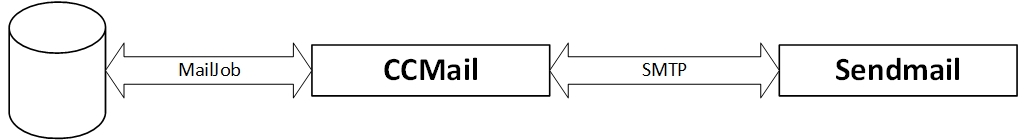
\includegraphics[scale=0.55]{teilsystem_ccmail.jpg} 
\caption{Teilsystem \emph{CCMail}}
\label{fig:ccmail-teilsystem}
\end{figure}
\ \newline
Der folgende Abschnitt wird die Schwächen der bestehenden Implementierung und deren Design analysieren. Die Ergebnisse dieser Analyse müssen bei der Erstellung des neuen Konzeptes mit einfließen und verhindern dass bereits gemachte Fehlentscheidungen sich wiederholen, sowie gute Ansätze weiterverfolgt werden.
\newline
\newline
Um das Design von \emph{CCMail} zu illustrieren wird im Folgenden näher auf die auf die Softwarekomponenten von \emph{CCMail} eingegangen. \emph{CCMail} besteht aus den folgenden Klassen:
\begin{enumerate}
	\item\emph{CCBasicEmail} ist die Basisklasse aller \emph{E-Mail}-Typen, die als abgeleitete Klassen von \emph{CCBasicEmail} implementiert wurden. Sie enthält alle bereitgestellten Funktionalitäten.
	\item\emph{CCMailingDao} ist die Schnittstelle zur Datenbank, welche alle SQL-Abfragen über alle \emph{E-Mail}-Typen hinweg enthält
	\item\emph{CCMailingFactory} ist die \emph{Factory-Method-Klasse} für das Erstellen von \emph{CCMailingDao} Objekten.
\end{enumerate}
\newpage

\subsection{Klasse \emph{CCBasicEmail}}
\label{sec:implementierung-ccbasic-mail}
Einleitend wird die Vererbungshierarchie der Klasse \emph{CCBasicEmail} diskutiert, welche die Basisklasse aller \emph{E-Mail}-Typen darstellt.
\begin{figure}[h]
\centering
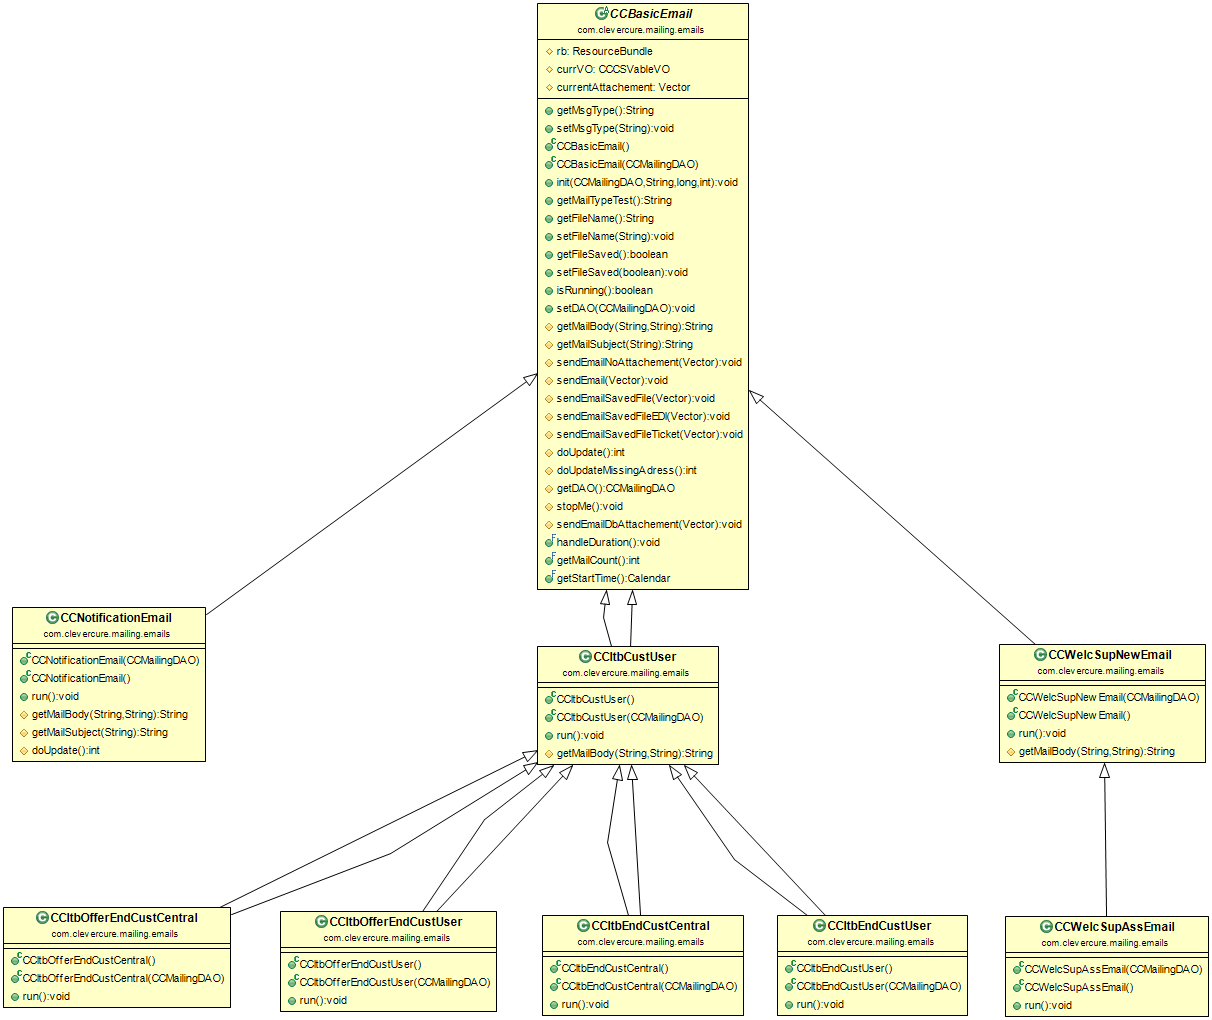
\includegraphics[scale=0.55]{class_diagram_basic_email.png} 
\caption{Auszug aus der Vererbungshierarchie von \emph{CCBasicEmail}}
\label{fig:klassen-hierarchie-ccbasicemail}
\end{figure}
\ \newline
Aus dem Klassendiagramm in Abbildung \ref{fig:klassen-hierarchie-ccbasicemail} lässt sich ableiten, dass die einzelnen \emph{E-Mail}-Typen als eigene Klassen abgebildet wurden. Somit ist jeder \emph{E-Mail}-Typ auch als eigene Java-Klasse abgebildet. 
\newline
\newline
Am Beispiel der Klasse \emph{CCItbCustUser} ist ersichtlich, dass neben dem Abbilden eines \emph{E-Mail}-Typs als eigene Java-Klasse man ebenfalls eine eigene Subvererbungshierarchie eingeführt hat, um \emph{E-Mail}-Typen, die sich in einem gemeinsamen Kontext befinden, zu gruppieren. Ob dies ein guter Ansatz ist, um kontextabhängige Ressourcen zu gruppieren, ist zu hinterfragen. Es gäbe hier andere Ansätze, wie man eine solche Gruppierung hätte realisieren können, die flexibler sind als eine Vererbungshierarchie. Eine Vererbungshierarchie ist starr und Änderungen an der Struktur können sich negativ auf die Gesamtstruktur auswirken. Ebenso produziert man so eine Vielzahl von Klassen, die gewartet werden müssen und die Struktur einer Subvererbungshierarchie lässt sich nur über ein Klassendiagramm darstellen und ist nicht aus dem Quelltext abzuleiten. Ebenso wird man bei den Vererbungshierarchien schnell an Grenzen stoßen, da hier nur gerichtete Graphen möglich sind und Mehrfachvererbung bei Klassen von Java nicht unterstützt wird. 
\newline
\newline
Mehrfachvererbung, auch wenn unterstützt, ist aber ohnedies zu vermeiden, da hier Kollisionen bei den Klassen Variablen und Methoden auftreten können. Außerdem wird durch Mehrfachvererbung die Komplexität der Klassenhierarchie nur unnötig erhöht und bringt daher keine Erleichterungen mit sich.

\subsection{Klasse CCItbCustUser}
Nachdem die Vererbungshierarchie von \emph{CCBasicEmail} diskutiert wurde, wird im Folgenden als Beispiel einer Implementierung von \emph{CCBasicEMail} die Implementierung der Klasse \emph{CCItbCustUser} angeführt. Diese Implementierung dient als Beispiel für die restlichen \emph{E-Mail}-Typ-Implementierungen, die nach dem selben Prinzip mit ähnlichem Umfang implementiert wurden. Im Abschnitt~\ref{sec:implementierung-ccbasic-mail} wurde behauptet, dass diese Ableitungen eingeführt wurden, um \emph{E-Mail}-Typen zu gruppieren. Man könnte aber auch annehmen, dass diese eigene Subvererbungshierarchie eingeführt wurde, um gemeinsame Funktionalitäten für die abgeleiteten \emph{E-Mail}-Typen zu kapseln. 
\newline
\newline
Folgender Quelltext illustriert, dass die Implementierungen der einzelnen \emph{E-Mail}-Typen hauptsächlich aus dem Erstellen der \emph{E-Mails} besteht, da der Versand bereits in der Klasse \emph{CCBasicEmail} implementiert wurde. Die Parameter für die Vorlage werden aus dem Resultat der spezifischen SQL-Abfrage in der Methode \emph{getMailBody} extrahiert und in der Nachricht bzw. der verwendeten Vorlage verwendet. Die erstellte Nachricht wird dann als Resultat geliefert. Das unterschiedliche Erstellen der \emph{E-Mails} ist also der Grund für das Abbilden der einzelnen \emph{E-Mail}-Typen als eigene Java-Klassen. Dieser Ansatz produziert viele Klassen, die in einer starren Hierarchie gebunden sind. Und dies nur um das Erstellen der eigentlichen \emph{E-Mail}-Nachricht in einer eigenen Java-Klasse zu kapseln. Es sei angemerkt, dass diese Klassen auch dazu verwendet um die \emph{E-Mail}-Typen zu aktivieren oder zu deaktivieren. Zu kritisieren ist hierbei, dass das Erstellen einer \emph{E-Mail} zu stark an einen \emph{E-Mail}-Typ gekoppelt ist und es hier an Abstraktion fehlt. Die \emph{E-Mail} werden immer nach dem selben Schema erstellt. Es gibt lediglich folgende Unterschiede:
\begin{itemize}
	\item SQL-Abfrage, welche die Daten aus der Datenbank bezieht.
	\item Die zugrunde liegende \emph{E-Mail}-Vorlage.
	\item Die Paramter für die zugrunde liegende \emph{E-Mail}-Vorlage.
	\item Der eindeutige Schlüssel, der den \emph{E-Mail}-Typ identifiziert.
\end{itemize}
\begin{program}
\begin{JavaCode}
public class CCItbCustUser extends CCBasicEmail {
	
	private Map cache = new HashMap();

	// empty constructor
	public CCItbCustUser() {
		super();
	} // end constructor
	
	// sets the used dao implementation
	public CCItbCustUser(CCMailingDAO dao) {
		super(dao);
	} // end constructor

	// The unique key for this email type
	@Override
	String getMailType() {
		return "ISCU";
	} // end getMailType
	
	// Thread.run method which creates and sends the email
	@Override
	public void run() {
		try {
			sendEmailNoAttachement(getDAO().getItbStartCustUserMailText());
		} catch (DAOSysException ex) {
			LOG.error("DAOSysException in CCItbCustUser.run: ", ex);
		} finally {
			stopMe();
		} // end try-catch-block
	} // end run
	
	// Method which creates the email body
	@Override
	protected String getMailBody(String bodyKey, String bodySQLKey)
		throws DAOSysException {
		int lanId   = ((CCItbVO)currVO).getLanguageId();
		int itbhId  = ((CCItbVO)currVO).getItbhID();
		String body = "";
		String key  = itbhId+"_"+lanId;
		if (cache.containsKey(key)) {
			body = (String)cache.get(key);
			LOG.debug("48: Got from cache key: "+key+" body: "+body);
		} else {
			Object[] allParams = getDAO().getItbCustData((CCItbVO)currVO, 19);
			MessageFormat form = new MessageFormat(rb.getString(bodyKey)
			                                         .trim());
	 		body               = form.format(params);
	 		cache.put(key, body);
	 		LOG.debug("48: DB access for the key: "+key+" got body: "+body);
		} // end if-else
		return body;
	} // end getMailBody
}
\end{JavaCode}
\caption{Implementierung \emph{CCItbCustUser}}
\label{fig:code-ccitbcustuser}
\label{CCItbCustUser.java}
\end{program}
\newpage
Die folgenden drei Methoden werden von den \emph{E-Mail}-Typ-Klassen implementiert:
\begin{enumerate}
	\item\emph{getMailType}: zum Bereitstellen eines eindeutigen Schlüssels, der diesen \emph{E-Mail}-Typ identifiziert.
	\item\emph{getMailBody}: zum Erstellen der \emph{E-Mail} aus einer Vorlage, welche mit Parametern befüllt wird.
	\item\emph{run}: Jeder \emph{E-Mail}-Typ wird in einem eigenen \emph{Thread} abgearbeitet. Dabei wird entschiedenen welche Art von \emph{E-Mail}-Versand genutzt wird. \emph{CCBasiEmail} stellt mehrere Implementierungen zur Verfügung z.B.:
	\begin{itemize}
		\item ohne Anhänge,
		\item mit Anhängen, welche über das lokale Filesystem zur Verfügung gestellt werden  und
		\item mit Anhängen, welche über externe Systeme zur Verfügung gestellt werden.
	\end{itemize}
\end{enumerate}
\ \newline
Der Quelltext aus Abbildung \ref{fig:code-ccitbcustuser} illustriert, dass die \emph{E-Mail}-Typen keine nennenswerte Logik haben, sondern lediglich für das Erstellen der \emph{E-Mail} verantwortlich sind. 

\subsection{Klasse CCMailingDao}
Im Gegensatz zur Strukturierung der \emph{E-Mail}-Typen hat man sich bei der Datenzugriffsschicht nicht dazu entschieden, diese kontextabhängig zu gruppieren. Hier wurden alle Datenbankabfragen in einer einzigen Schnittstelle spezifiziert, ohne Rücksichtnahme auf deren Kontext.
\newline
\begin{figure}[h]
\centering
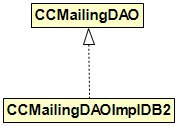
\includegraphics[scale=0.55]{class_diagram_mailing_ao.png} 
\caption{Vererbungshierarchie von \emph{CCMailingDao}}
\label{fig:klassen-hierarchie-ccmailingdao}
\end{figure}
\ \newline
Die Vererbungshierarchie aus Abbildung \ref{fig:klassen-hierarchie-ccmailingdao} ist sehr einfach, da man sich hier nicht für eine Aufteilung der Datenbankzugriffsschicht für die einzelnen \emph{E-Mail}-Typen entschieden hat. Dabei ist zu bemängeln, dass sich alle Datenbankabfragen über alle \emph{E-Mail}-Typen hinweg befinden und man es versäumt hat hier Schnittstellen einzuführen, welche die kontextabhängigen Datenbankabfragen spezifizieren,  also eine Schnittstelle für jeden \emph{E-Mail}-Typ. Mit einer Aufteilung auf mehrere Schnittstellen hätte man die Wartung der Datenbankabfragen vereinfacht. Mit dem Ansatz der Aufteilung auf mehrere Schnittstellen, wäre man einerseits gezwungen Präfixe für die Methodennamen einzuführen, da Namenskollisionen sehr wahrscheinlich sind, und andererseits muss man darauf Acht geben, bestehende Implementierungen bei einem Restrukturieren einer oder mehrerer kontextabhängigen Implementierungen nicht zu verändern. 
\newline
\newline
Alle Implementierungen nutzen dieselben Ressourcen und müssen daher auf den kleinsten gemeinsamen Nenner zusammengeführt werden, oder man führt wiederum eigene Ressourcen ein, die sich durch ihren Namen unterscheiden. 
\newline
\newline
Eigene Schnittstellen und Implementierungen je \emph{E-Mail}-Typ hätten es ermöglicht, für jeden dieser \emph{E-Mail}-Typen Ressourcen zur Verfügung zu stellen, die nur dieser \emph{E-Mail}-Typ verwendet. Mann hätte Flexibilität erhalten und hätte sich trotzdem auf eine gemeinsame Basis einigen können. 
\newline
\newline
Der Ansatz, die Implementierungen von \emph{CCMailingDAO} für verschiedene Datenbanken zu zur Verfügung zu stellen, ist an sich gut, jedoch hätte man sich mit der Nutzung von ORM \emph{(Object Relational Mapping)} das Leben erleichtern können, da ein \emph{ORM-Provider}, wie z.B.: \emph{Hibernate}, bereits die zugrunde liegende Datenbank abstrahiert. Datenbank-spezifische SQL-Anweisungen und Funktionalitäten werden zwar von den \emph{ORM-Providern} nicht zur Verfügung gestellt, jedoch sind solche spezifischen Teile in \emph{CCMail} nicht zu finden. Die Entscheidung, sich hier auf native SQL-Abfragen zu stützen, bringt das Problem mit sich, dass die zugrunde liegende Datenbank nicht von der Anwendung abstrahiert ist und man sich so an eine spezielle Datenbankimplementierung bindet.

\subsection{Klasse \emph{CCMailingDaoFactory}}
Zu kritisieren ist auch die Art und Weise wie ein Objekt von \emph{CCMailingDao} erzeugt wird. Man nutzt hier das Softwaremuster \emph{Factory-Method}, jedoch wird statisch die zu verwendende Implementierung in \emph{CCMailingDaoFactory} definiert, was das Austauschen der Implementierung zur Laufzeit unmöglich macht. Man hätte dies konfigurierbar machen sollen, z.B über eine Konfigurationsdatei, die den zu verwendenden Implementierungsnamen zur Verfügung stellt.
\begin{figure}[h]
\centering
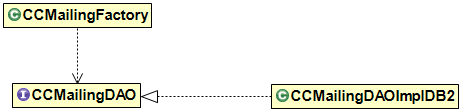
\includegraphics[scale=0.5]{class_diagram_mailing_dao_factory.png} 
\caption{\emph{CCMailingDaoFactory} für \emph{CCMailingDao}}
\label{fig:klassen-hierarchie-ccmailingfactory}
\end{figure}
\ \newline 
Im Buch \emph{Refactoring to patterns} \cite[72]{refactoreToPatterns} wird als Nachteil einer \emph{Factory-Method} die erhöhte Komplexität des Designs genannt, wenn eine direkte Instanziierung auch genügen würde. Nachdem die Instanziierung in der Basisklasse \emph{CCBasicEmail} erfolgt und die Ableitungen die Objekte über eine Get-Methode oder die geschützte Datenkomponente erreichen können, hätte man auf diese \emph{Factory} verzichten können, da die Abstraktion bereits über die Basisklasse \emph{CCBasiEmail} erreicht wurde. Somit ist der Formalparameter der Konstruktoren vom Typ \emph{CCMailingDAO} sinnlos und der Grund warum man dies eingeführt hat, ist nicht ersichtlich. Man hätte die Verwaltung der \emph{CCMailingDAO} Objekte in der abstrakten Basisklasse \emph{CCBaisEmail} halten sollen, ohne die abgeleiteten Klassen damit zu verschmutzen. 
\newline 
\newline
Zusätzlich befinden sich die Quelltexte der Schnittstellen zusammen mit ihrer Implementierungen in einem einzigen Projekt. Dies ist auch als ein halbherziger Versuch zu werten, die Implementierung von \emph{CCMailingDao} austauschbar zu machen. Man hätte hier die Quelltexte der Schnittstellen und der Implementierungen auf eigene Projekte aufteilen sollen. Somit hätte man die Abhängigkeit zu den konkreten Implementierungen der Schnittstellen vermieden und hätte sich nicht der Gefahr ausgesetzt, dass ein Entwickler sich direkt auf eine Implementierung beziehen könnte und daher immer gezwungen wäre, mit den Schnittstellen zu arbeiten.

\section{\emph{CCMail}-Datenbank}
\label{sec:ccmail-datanbank}
Abschließend wird der Aufbau des Datenbankschemas betrachtet, welches die Kernkomponente des Systems aus der Sicht von \emph{CCMail} darstellt. Bei diesem Schema wurde auf Fremdschlüssel verzichtet, was grundsätzlich nur in Spezialfällen anzuraten ist.
\newline
\newline 
Im Buch \emph{Refactoring Database} \cite[213]{refactoreDatabase} wird als Argument für nicht verwendete Fremdschlüssel die Performanz genannt, wobei in diesem Fall diese Begründung nicht hält. Die beiden Anwendungen \emph{CleverWeb} und \emph{CleverInterface} erstellen lediglich einzelne oder wenige \emph{MailJob}-Einträge auf einmal, und \emph{CCMail} ist die einzige Anwendung, die diese \emph{MailJob}-Einträge einmalig ausliest und verarbeitet. Also muss die Performance ohnehin kein Problem darstellen, da hier keine Vielzahl von TeilnehmerInnen und die keine Konkurrenz nicht geben ist. Das Problem von nicht verwendeten Fremdschlüsseln wird in \emph{Refactoring Databases} \cite[213]{refactoreDatabase} wie folgt beschrieben:
\newpage
\begin{quote}
\emph{The fundamental tradeoff is performance versus quality: Foreign key constraints ensure the validity of the data at the database level at the cost of the constraint being enforced each time the source data is updated. When you apply Drop Foreign Key, your applications will be at risk of introducing invalid data if they do not validate the data before writing to the database.}
\end{quote}
Es müssen also die Anwendungen selbst die Konsistenz der Daten gewährleisten, ansonsten könnten inkonsistente Datenbestände in der Datenbank entstehen, die nachträglich schwer zu identifizieren und zu bereinigen sind. Die Frage ist, ob dieser Ansatz ein guter ist?
\newline
\newline
Wie in Abbildung \ref{fig:ccmail-db-schema} ersichtlich, wurden die Spalten der Tabellen mit einem Präfix versehen, der eindeutig über das gesamte Datenbankschema ist. Mann sollte wissen, dass es ausreicht, dass die Spaltennamen eindeutig innerhalb des Kontexts einer Tabelle sind und nicht global über das gesamte Datenbankschema. Ebenso erkennt man, dass folgende Tabellen Fremdschlüssel definieren: 
\begin{itemize}
	\item\emph{MAIL\_JOB\_ATTACHMENT\_CONTAINERS}:
	\newline
	ist die Tabelle, welche die gebündelten Anhänge (*.zip) für einen \emph{MailJob} repräsentiert.
	\item\emph{MAIL\_ATTACHMENT\_CONTAINER}:
	\newline
	ist die Tabelle, welche ein Bündel von Anhängen für einen \emph{MailJob} repräsentiert.
	\item\emph{MAIL\_ATTACHMENT\_CONTAINER\_ATTACHMENT}:
	\newline
	ist die Tabelle, welche einen Anhang eines \emph{MailJob} repräsentiert.
	\item\emph{MAIL\_ATTACHMENT\_PARTS}:
	\newline
	ist die Tabelle, welche die partitionierten und in \emph{BASE64} kodierten Daten der Anhänge des \emph{MailJob} repräsentiert.
	\item\emph{MAIL\_ATTACHMENT}:
	\newline
	ist die Tabelle, welche einen Anhang eines \emph{MailJob} repräsentiert. 
	\item\emph{MAIL\_JOB\_ATTACHMENT}:
	\newline
	ist die Tabelle, welche die Anhänge eines \emph{MailJob} repräsentiert.
\end{itemize}
\ \newline
Diese Tabellen wurden nachträglich hinzugefügt und man hat den Ansatz des Verzichts auf Fremdschlüssel offensichtlich aufgegeben. Diese Tabellen werden dazu verwendet, um Datei- Anhänge von \emph{E-Mail} zu verwalten, die bereits bei der Erstellung des \emph{MailJobs} vorhanden sind. Dies war eine Umgehungslösung und darf so auch nicht mehr angewandt werden, da hier die Dateien kodiert in Base64 (\emph{Codepage} unabhängige ASCII- Zeichenfolge) gehalten werden und die Datenbank unnötig mit Daten belasten. Die Dateien müssten nur als Referenzen in der Datenbank präsent sein.
\ \newpage
\subsection{Datenbankschemata von \emph{CleverMail}}
Folgende Abbildung \ref{fig:ccmail-db-schema} illustriert das Datenbankschema von \emph{CCMail}.
\begin{figure}[H]
\centering
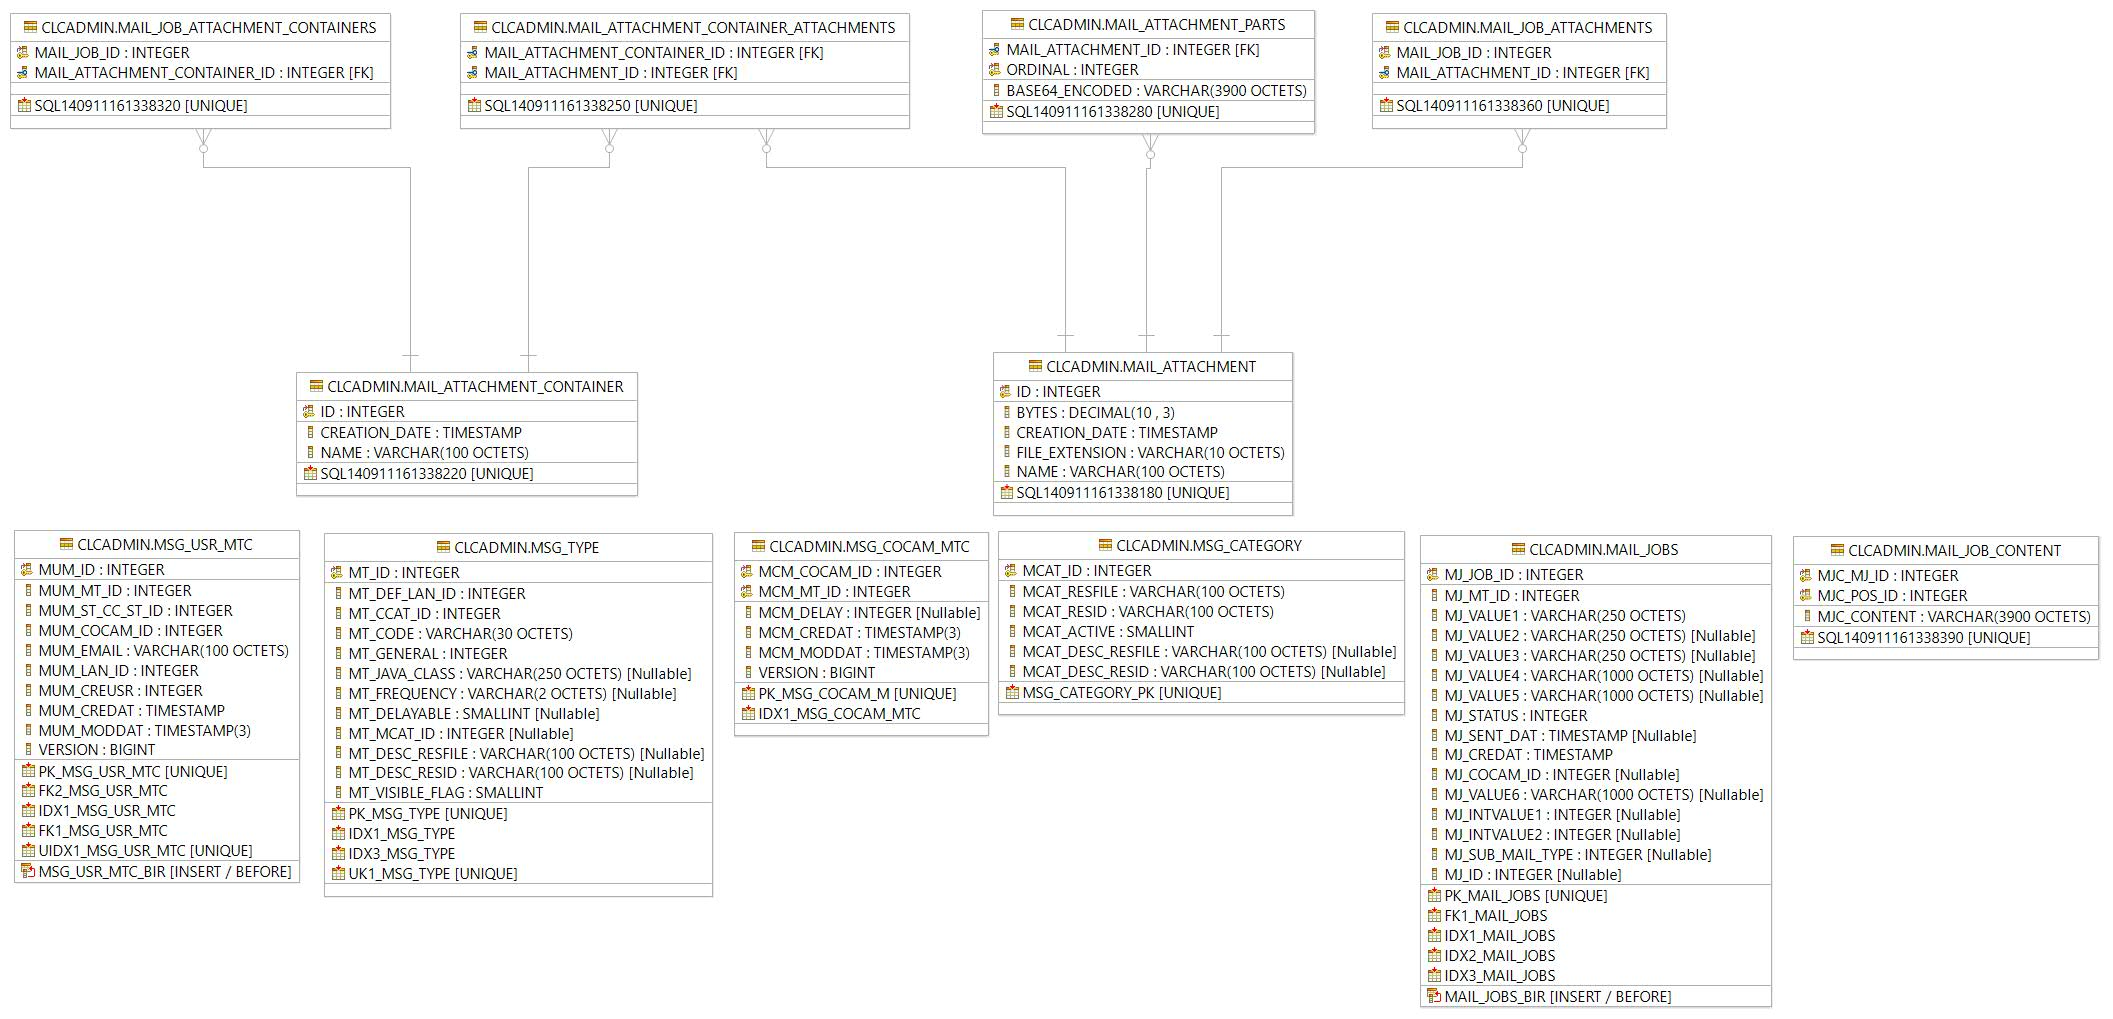
\includegraphics[angle=90,scale=0.4]{ccmail_db_schema.jpg} 
\caption{Datenbankschema \emph{CCMail}}
\label{fig:ccmail-db-schema}
\end{figure}
Mit den Betrachtungen des Datenbankschemas von \emph{CCMail} ist die Analyse von \emph{CCMail} abgeschlossen. Bei der Analyse wurden einige Probleme und Fehlentscheidungen von \emph{CCMail} identifiziert wie z.B.:
\begin{itemize}
	\item Die Vererbungshierarchie der \emph{Mail}-Typen.
	\item Die Statische \emph{Mail}-Vorlagen.
	\item Der Verzicht auf Datenbank-Fremdschlüssel.
	\item Die global eindeutigen Namen der Tabellenspalten.
\end{itemize}
\ \newline
Die Ergebnisse der Betrachtungen stellen eine Grundlage für die Konzipierung von \emph{CleverMail} dar. Folgendes Kapitel wird sich neben der Konzeption von \emph{CleverMail} auch mit neuen Technologien und Bibliotheken befassen, die für \emph{CleverMail} Anwendung finden könnten. 
\chapter{CleverMail}
\label{cha:clevermail}
In diesem Kapitel wird nun das Konzept von \emph{CleverMail} behandelt, welches die bestehende Anwendung \emph{CCMail} ablösen soll. Nachdem die Betrachtungen und Analysen von \emph{CCMail} abgeschlossen sind und einige Fehlentscheidungen ausgemacht wurden kann man sich jetzt dem Konzept für \emph{CleverMail} zuwenden. Im Gegensatz zu \emph{CCMail} wird aus der Sicht von \emph{CleverMail} das Gesamtsystem aus mehr Anwendungen bestehen, die in der Lage sein müssen E-Mail-Nachrichten zu versenden. Über die Zeit ist das GEsatmsystem \emph{clevercure} angewachsen und es wurden neue Anwendungen hinzugefügt, die Aufgrund der Architektur von \emph{CCMyail} nicht eingebunden werden konnten bzw. man sich dazu entschieden hat die Einbindung zu unterlassen.
\newline
\newline
Folgende Auflistung zeigt alle Anwendungen, die \emph{CleverMail} nutzen werden:
\begin{enumerate}
	\item\emph{CleverWeb}
	\newline
	Die Web-Anwendung für den webbasierten Zugriff auf das System
	\item\emph{CleverInterface}
	\newline
	Die Schnittstellen Anwendung für den Datenimport/-export
	\item\emph{CleverSupport (neu)}
	\newline
	Die Web-Anwendung für die Support Abteilung
	\item\emph{CleverDocument (neu)}
	\newline
	 Das Dokumentenmanagementsystem welches von allen Anwendungen genutzt wird
\end{enumerate}
Im Gegensatz zu \emph{CCMail} soll \emph{CleverMail} nicht als Konsolenanwendung implementiert werden sondern soll als Enterprise-Anwendung implementiert, welche als eigenständige Anwendung in einem JEE7-Applikationsserver betrieben wird.
\newpage
Mit dieser Art von Anwendung stehen \emph{CleverMail} eine Vielzahl von Features und Frameworks zur Verfügung wie z.B.: 
\begin{enumerate}
	\item JAX-RS 2.0 (Java API for RESTful Webservices)
	\item EJB 3.1 (Enterprise-Java-Bean)
	\item JPA 2.1 (Java-Persistence-API)
	\item JTA 1.2 (Java-Transaction-API)
	\item JSF 2.2 (Java-Server-Faces)
	\item uvm.
\end{enumerate}
Dies Features werden es erlauben die Anwendung \emph{CleverMail} so flexibel wie möglich zu gestalten, bringen aber auch ein erhöhtes Maß an Komplexität beim Design mit sich. Martin Fowler führt in seinem Buch \emph{Patterns of Enterprise Application Architecture}\cite[5-6]{patternsOfEnterprise} einige Beispiel für Enterprise-Anwendungen an um zu illustrieren dass jede dieser Anwendungen seine eigenen Probleme und Komplexität mit sich bringt und sich daher die Architektur einer Enterprise-Anwendung nicht einordnen und quantifizieren lässt. Daher ist beim Erstellen einer Architektur einer Enterprise-Anwendung der konkrete Nutzung zu berücksichtigen. Der Prozess der Konzeption einer Architektur ist ein kreativer Prozess wobei Konzepte, Best-Practise usw. nur als Unterstützung anzusehen sind und es keinen echten Leitfaden gibt an den man sich orientieren kann. Die Architektur wird stark von der konkreten Anwendung beeinflusst. Daher kann sich die Architektur je nach Anwendung stark unterschieden.
\newpage
\section{Systemaufbau}
Im Gegensatz zum Systemaufbau aus der Sicht von \emph{CCMail}, beschrieben in \ref{sec:ccmail-systemaufbau}, soll die Datenbank nicht mehr als Schnittstelle zwischen den Anwendungen und \emph{CleverMail} fungieren. Die Datenbank soll weiterhin ein zentraler Bestandteil von \emph{CleverMail} sein jedoch soll diese von den Anwendungen abstrahiert werden. Damit erreicht man dass die Anwendungen eine einheitliche Schnittstelle nutzen und nicht ihrerseits eigene Implementierungen warten müssen.
\begin{figure}[h]
\centering
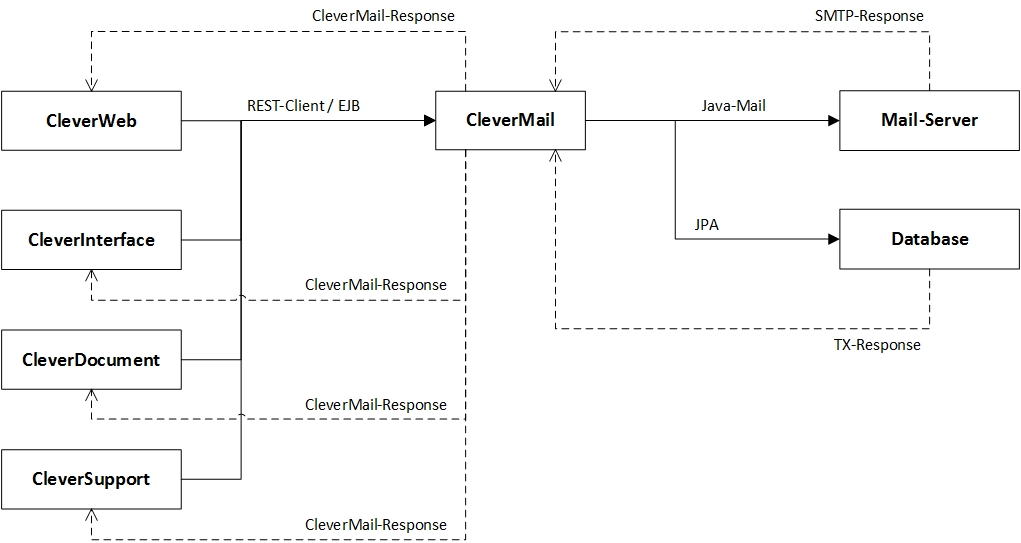
\includegraphics[scale=0.58]{clevermail_systemaufbau.jpg} %{CS0031}
\caption{Systemaufbau und Integration von \emph{CleverMail}}
\label{fig:clevermail-system-und-integration}
\end{figure}
\ \newline
Wie in der Abbildung \ref{fig:clevermail-system-und-integration} illustriert soll als zentrale Schnittstelle \emph{CleverMail} bzw. dessen implementierte Client-API fungieren wobei diese CLient-API sich wie folgt ausprägen könnte:
\begin{enumerate}
	\item\emph{REST-Client}
	\newline
	Eine REST-Schnittstelle zu einen REST-Webservice über den die zur verfügung gestellten Funktionalitäten genutzt werden können.
	\item\emph{EJB}
	\newline
	Ein EJB-Bean welches die zur Verfügung gestellten Funktionalitäten bereitstellt.
\end{enumerate}
\ \newline
\emph{CleverMail} seinerseits ist für die Persistenzschicht und das versenden der E-Mail-Nachrichten verantwortlich und trennt diese Aufgaben vollständig von den Anwendungen. So kann die Wartung nur an einer stelle erfolgen und muss nicht über alle Anwendungen hinweg erfolgen. In den Anwendungen würden nur noch Änderungen an den Schnittstellen Eingriffe erfordern.
\newpage
Dieser Ansatz würde das Problem der eigens implementierten Datenbankzugriffe \ref{sec:ccmail-systemaufbau} lösen. Ein Problem könnten hier etwaige technologische Unterschiede darstellen wie z.B.:
\begin{enumerate}
	\item REST nicht verfügbar
	\item EJB nicht verfügbar
	\item Falscher Source-Level
\end{enumerate}
\ \newline
Obwohl diese Probleme auftreten könnten kann zumindest gewährleistet werden, dass alle Anwendungen dieselbe Schnittstelle und dasselbe Domain-Model verwenden, selbst wenn eigene Implementierungen erforderlich sind. Diese Implementierungen würden eine Softwarekomponente von \emph{CleverMail} darstellen und währen auch Teil dieser Anwendung und dürfen nicht von den Anwendungen selbst bereitgestellt werden.
Diese technologischen Unterschiede könnten wie folgt gelöst werden.
\begin{enumerate}
	\item\emph{REST}
	\newline
	Integration von JAX-RS 2.0 
	\item\emph{EJB}
	\newline
	Integration eines EJB-Containers, zur Verfügung stellen eines Wrappers oder eine eigene Implementierung des spezifizierten Interfaces
\end{enumerate}
\subsection{REST-Client}
Eine REST-Client API, welche sich mit JAX-RS 2.0 einfach realisieren lässt, würde ein hohes Maß an Abstraktion bieten, nur eine geringe Kopplung aufweisen und wenig Abhängigkeiten in der Anwendung erfordern. Dies steht aber gegenüber dass REST-Services zustandslos sind und sich daher implizit nicht in Datebank 
Transaktionen einbinden lassen. Dies könnte aber erforderlich sein wenn eine E-Mail nur dann angelegt und versendet werden darf wenn die Transaktion erfolgreich abgeschlossen wurde (z.B.: Anlegen einer Bestellung). Würde über den REST-Service eine E-Mail Nachricht angelegt werden. Für einen REST-Service startet eine Transaktion mit dessen Aufruf und endet mit dem Übermitteln der Response oder wenn die Aktion abgeschlossen wurde (asynchron).
\newpage
Für diese Problem gibt es eine Lösung in Form eines Konzeptes mit der Bezeichnung Try-Confirm-Cancel (TCC).
\begin{figure}[h]
\centering
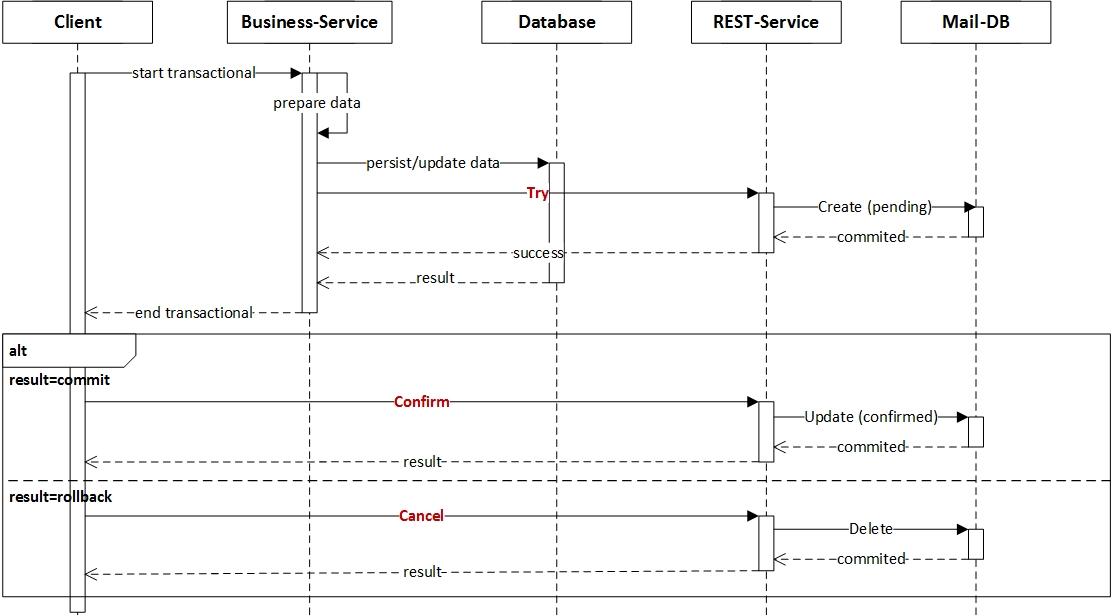
\includegraphics[scale=0.5]{try_confirm_cancel.jpg} %{CS0031}
\caption{Beispiel einer Transaktion mit TCC}
\label{fig:clevermail-rest-tcc}
\end{figure}
\ \newline
Mit diesem Konzept müsste der REST-Service den Zustand persistent halten aber als \emph{unconfirmed} markieren, damit dieser in keiner Verarbeitungslogik miteinbezogen wird. Nachdem erfolgreichen Abschluss der Transaktion auf der Client-Seite muss dieser durch den REST-Service persistent gehaltenen Zustand bestätigen und im Falle eines Fehlers abbrechen. Dies würde zwei Aufrufe zu REST-Services verursachen. Ebenfalls sollte die Transaktion über einen Transaktionskoordinator auf der REST-Seite kontrolliert werden, was wieder einen Mehraufwand bedeutet. Dieser Transaktionskoordinator ist dafür verantwortlich die REST-Services, die Teil einer logischen Transaktionen sind,  zu managen. Mit \emph{TCC} besteht auch die Gefahr das eine Heuristic-Exception auftritt. Beim Auftreten einer solchen Exception würden inkonsistente Datenbestände auf der Datenbank entstehen, da es sein könnte das nicht alle REST-Services ein Rollback durchgeführt haben.
\newline
\newline
Diese Probleme bedeuten aber nicht dass REST-Services nicht in Frage kommen. Lediglich für transaktionale Operationen scheinen sie ungeeignet bzw. der Aufwand der betrieben werden muss zu hoch. Ein weiteres Problem könnte die Erreichbarkeit dieser REST-Services sein. Sollte dieser einmal ausfallen oder im Falle eines Deployments nicht erreichbar sein so müsste man eine Rückversicherung haben und die zu erstellenden E-Nachrichten anderweitig zwischenspeichern wie z.B.: in Form einer Textdatei, welche die Daten als JSON enthält.
\newline
\newline
Diese Onlinepublikation \cite{atomikosTcc} beschreibt den Prozess von \emph{TCC} mit mehreren involvierten REST-Services sehr gut und detailliert.
\subsection{EJB}
Sollte eine Anwendung über EJB mit \emph{CleverMail} kommunizieren so würde hierbei eine starke Kopplung und starke Abhängigkeiten entstehen, da hier mehr Ressourcen benötigt werden. Ebenso könnte im Gegensatz zu einem REST-Client keine eigene Datenbank genutzt werden, da hier ein Zweiphasen-Commit erfolgen müsste. Natürlich würde diese Möglichkeit bestehen aber auch hier wäre man der Gefahr von Heursitc-Exceptions ausgesetzt.
\begin{figure}[h]
\centering
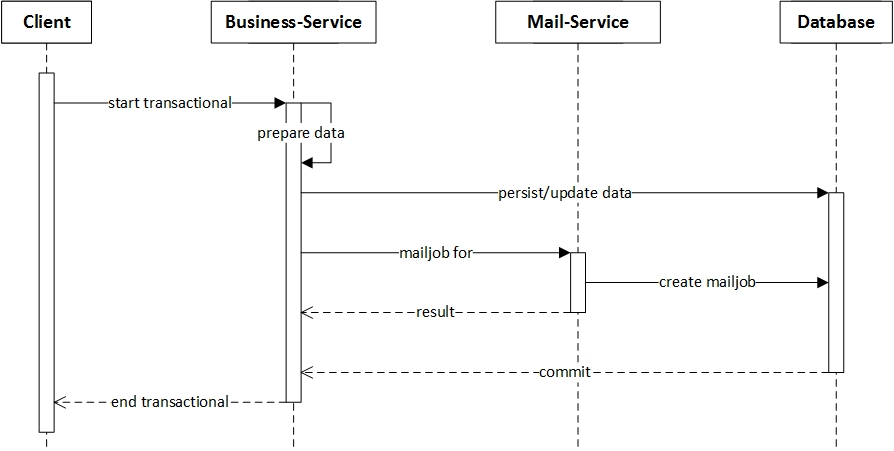
\includegraphics[scale=0.5]{clevermail-ejb-transaktion.jpg} %{CS0031}
\caption{Beispiel einer EJB (JTA) Datenbanktransaktion}
\label{fig:clevermail-rest-tcc}
\end{figure}
\ \newline
In diesem Fall würde das Anlegen einer E-Mail in derselben Transaktione erfolgen und würde daher auch im Falle eines Roolbacks entfernt werden. Dies ist sicher die angenehmste Art und Weise um E-Mails anzulegen, da hier keine besonderen Mechanismen implementiert werden müssten um die Datenkonsistenz zu gewährleisten. Hierbei währen die E-Mail-Nachrichten auch Teil einer wohl definierten Transaktion.
\newline
\newline
Wie hier \ref{cha:clevermail} angemerkt können technologische Probleme auftreten wenn z.B.: eine Anwendung kein \emph{EJB} und/oder \emph{JPA} unterstützt. Hierbei müsste man eine eigene Implementierung erstellen, die zumindest Teil von \emph{CleverMail} sein sollte.
\newline
\newline
Dieser transaktionale Ansatz unterschiedet sich nicht von dem in \emph{CCMail} bereits implementierten jedoch sollen hier die von \emph{CleverMail} zur Verfügung gestellten implementierten Ressourcen verwendet werden. Diese Ressourcen sollten auch im Backend der REST-Services von \emph{CleverMail} angewandt werden, da auch hier die Persistenz der E-Mails gewährleistet werden muss. 
\newpage
\chapter{Prozesse}
\label{cha:clevermail-prozesse}
Diese Kapitel behandelt die Prozessspezifikationen von \emph{CleverMail}. Hierbei wird das Augenmerk auf den Mailversand gelegt. Grundlegend wird sich der E-Mail-Versand dadurch unterschieden, dass hier mehrere Ebenen involviert sind, bevor eine E-Mail-Nachricht bereit zum Versand ist. Vom grundlegenden Konzept wird sich gegenüber \emph{CCMail} nicht viel ändern. Es soll immer noch E-Mail-Typen geben, die aber jetzt nicht nur intern konfigurierbar sein sollen sondern ebenfalls durch die Kunden selbst konfiguriert und gesteuert werden können. Hierbei sollen folgende Konfigurationsmöglichkeiten zur Verfügung stehen.
\begin{enumerate}
	\item Definition von Schedules
	\item Definition eigener E-Mail-Vorlagen
	\item Konfiguration der Steuerbarkeit von E-Mail-Typen durch Lieferanten (darf aktivieren/de-aktivieren)
	\item Definition eines Haftungsausschluss 
	\item Definition von Standard Datei Anhängen
	\item Steuerbarkeit von E-Mail-Typen für spezifischen Lieferanten
	\item Konzernübergreifende Konfiguration
	\item Definition eigener E-Mail-Typen
	\item Konfiguration der Historie der E-Mail-Nachrichten
\end{enumerate}
\ \newline
Zur Zeit stehen diese Features, wenn vorhanden, nur intern zur Verfügung. Die Kunden haben lediglich die Möglichkeit einzelne E-Mail-Typen zu aktivieren oder zu de-aktivieren. Diese E-Mail-Typen können aber mehrere E-Mail-Nachrichten beinhalten. Das Grundlegende Ziel ist das die Kunden mehr Kontrolle und Konfigurationsmöglichkeiten über die zur Verfügung gestellten E-Mail-Typen erhalten. Es wird hier aber auch solche E-Mail-Typen geben, bei denen diese Konfigurationsmöglichkeiten eingeschränkt werden. Nichts desto trotz soll der Kunde in der Lage sein, den E-Mail-Verkehr seiner E-Mail-Nachrichten besser zu steuern.
\newpage
\section{E-Mail-Versand}
\begin{figure}[h]
\centering
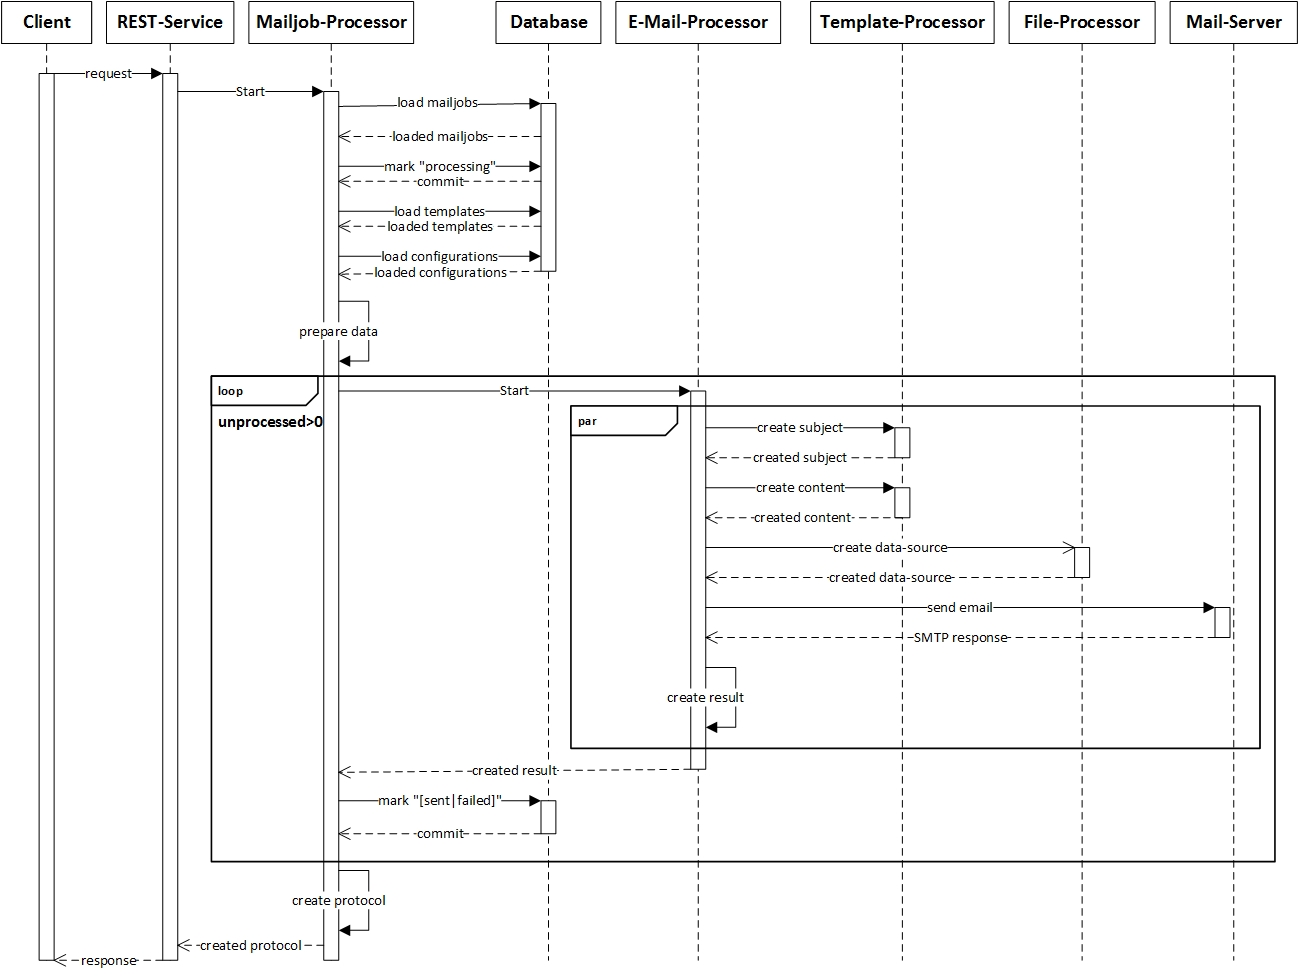
\includegraphics[angle=90, scale=0.6]{clevermail-email-versand.jpg} %{CS0031}
\caption{Prozess des E-Mail-Versands}
\label{fig:clevermail-email-versand}
\end{figure}
\ \newpage
Die Abbildung \ref{fig:clevermail-email-versand} soll den Prozess des E-Mail-Versands veranschaulichen und illustriert die involvierten Komponenten, die involviert sind um eine E-Mail-Nachricht zu erstellen. In diesem Beispiel wird der Prozess über einen REST-Service gestartet, der in diesem Fall den Prozess synchron abarbeitet und anschließend eine Response in Form eines erstellten Reports zurückliefert. Der REST-Service ist hierbei als optional anzusehen, da dieser Prozess auch anderweitig ausgelöst werden könnte. Nachdem sich dieser Prozess nicht in einer Transaktion eines Client befinden muss würde sich hier eine REST-Schnittstelle anbieten.
\newline
\newline
Folgende sei der Prozess in grobe Schritte unterteilt angeführt und beschrieben.
\subsection{Daten Aufbereitung}
Nachdem der Prozess gestartet wurde sollen die zu verarbeitenden E-Mail-Nachrichten aus der Datenbank ausgelesen und als \emph{Processing} markiert. Im Punkt \ref{sec:ccmail-gesamtprozess} wurde angemerkt, dass das Problem bestand ,dass die in Verarbeitung stehenden \emph{MailJob} Entitäten nicht als solche markiert wurden und daher eine parallele Verarbeitung durch mehrere Prozesse nicht möglich war. Dieses Problem besteht in diesem Fall nun nicht mehr. Nachdem die \emph{MailJob} geladen wurden sollen die zugrunde liegenden E-Mail-Vorlagen geladen werden. Hierbei würde sich ein Cache-Mechanismus auszahlen, da die E-Mail-Vorlagen Versionen definieren und sich innerhalb einer Version nicht ändern dürfen. Anschließend sollen die kundenspezifischen Konfigurationen geladen werden. Aus diesen Daten sollen Modelle erstellt werden, die in weitere Folge dazu verwendet werden sollen die E-Mail-Nachrichten zu erstellen.
\subsection{Erstellen der E-Mail-Nachrichten}
Aus den Modellen sollen die E-Mail-Nachrichten erstellt werden. Hierbei wird dieser Prozess in drei Schritte unterteilt.
\begin{enumerate}
	\item\emph{Erstellen des Betreff}
	\newline
	Der Betreff wird aus einer E-Mail-Vorlage erstellt und mit Daten befüllt sollten in der Voralge Parameter definiert worden sein
	\item\emph{Erstellen der Nachricht}
	\newline
	Die Nachricht wird aus einer E-Mail-Vorlage erstellt und mit Daten befüllt sollten in der Voralge Parameter definiert worden sein
	\item\emph{Erstellen der DataSoruces}
	\newline
	Sollten Datei Anhänge definiert worden sein, so werden diese in Form von einer oder mehrerer DataSoruce Instanzen in die E-Mail-Nachricht angefügt.
\end{enumerate}
\ \newline
Die Verarbeitung der E-Mail-Vorlagen soll in einer Komponente mit dem Name \emph{Template-Processor} erfolgen. Nachdem die Werte der verwendeten Vorlagenparameter beim Erstellen eines \emph{MailJob} in der Datenbank gespeichert wurden können diese hier angewandt werden.
\newline
\newline
Die Verarbeitung der Datei Anhänge soll in einer Komponente mit dem Namen \emph{File-Processor} erfolgen, die die verlinkten Datei Anhänge in Form von \emph{DataSource} Instanzen der E-Mail-Nachricht zur Verfügung stellt. Beim Versand würde die E-Mail-Nachricht den Datei Anhang über diese \emph{DataSource} Instanz laden. Hierbei sollen die Dateien in Form von Links aus dem Dokumentenmanagementsystem \emph{CleverDocument} geladen werden. Es soll keine Dateien in Form von Base64-Zeichenketten in der Datenbank mehr geben. Es könnten hierbei verschiedene \emph{DataSource} Implementierungen zur Verfügung gestellt werden, die die Dateien aus verschiedenen Quellen über die verschiedensten Protokolle laden können (z.B.: REST, SOAP, HTTP, usw.).
\subsection{E-Mail versenden}
Der E-Mail-Versand sowie das Erstellen der E-Mail-Nachricht sollte hierbei asynchron erfolgen, da eine sequenzielle Verarbeitung die Performance negativ beeinflussen würde. Nach dem erfolgreichen oder fehlgeschlagenen Versand einer E-Mail-Nachricht soll dieser Status in Form eines Resultates zurückgeliefert werden. Hierbei ist vor allem die SMTP-Response wichtig, die auf jeden Fall gespeichert werden soll damit der Kunde nachvollziehen kann wie der E-Mail-Versand seiner E-Mail abgearbeitet wurde und warum die E-Mail nicht zugestellt werden konnte. Ein fehlgeschlagener Versand könnte folgende Ursachen haben:
\begin{enumerate}
	\item Datei kann nicht geladen werden (nicht vorhanden, Timeout,...)
	\item Mail-Server des Empfängers nicht erreichbar
	\item E-Mail-Server nimmt Nachricht nicht an
	\item uvm.
\end{enumerate}
\ \newline
Es kann unzählige Ursachen haben warum eine E-Mail-Nachricht nicht zugestellt werden kann. Die trifft vor allem auf den E-Mail-Servers des Empfängers zu, auf dessen Konfiguration kein Einfluss genommen werden kann.
\newpage
\section{E-Mail-Vorlagenparameter}
Ein weiterer wichtiger Aspekt stellen die Vorlagenparameter und deren Verwaltung dar. Die Bereitstellung von Vorlagenparametern soll den AnwenderInnen die Möglichkeit bieten auf kontextabhängige Daten in einer E-Mail-Vorlage zugreifen zu können. Dadurch soll die Flexibilität erhöht werden und die AnwenderInnen sollen mehr Freiheiten beim Erstellen einer E-Mail-Vorlage bekommen. Diese Parameter müssen hierbei von den EntwicklerInnen innerhalb eines Kontextes zur Verfügung gestellt werden, wobei hier auch ein Entwicklungsaufwand besteht. Diese Parameter müssen beim Verarbeiten einer E-Mail-Vorlage aus dem aktuellen Kontext ausgelesen werden. Dabei können die Daten aus verschiedenen Objekten oder sogar Objektgraphen kommen. Dies bedeutet das diese Parameter über eine spezielle Implementierung ausgelesen werden müssen, die auch zukünftig gewartet werden muss. Ebenso werden diese Parameter in verschiedenen Softwarekomponenten verwendet die sich in verschiedenen Laufzeitumgebungen genutzt werden können. Daher wird es erforderlich sein diese Parameter in einem spezifizierten Model oder über definierte Zuordnungen von einem Model in ein anderes Model zu überführen.
\begin{figure}[h]
\centering
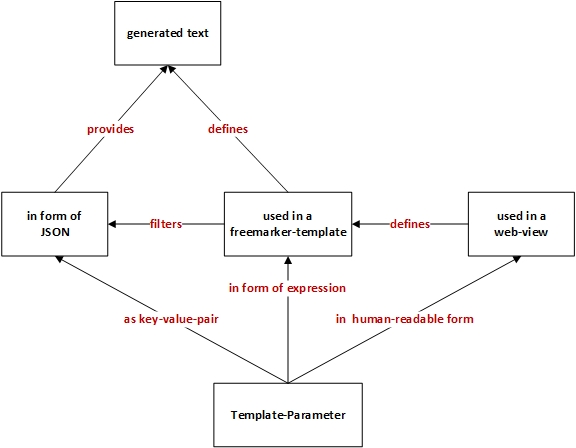
\includegraphics[scale=0.6]{clevermail_template_parameter.jpg}
\caption{Verwendung Vorlagenparameter}
\label{fig:clevermail-template-parameter}
\end{figure}
\ \newline
Wie in der Abbildung \ref{fig:clevermail-template-parameter} illustriert werden die Vorlagenparameter in mehreren Kontexten verwendet. Dadurch stellt sich die Frage wie diese Parameter adressiert werden. Man könnte eine Zuordnung in jedem Verwendungskontext erstellen, also jeder Kontext bekommt sein eigenes Model. Dadurch würde man sich zwar lose and die Vorlagenparameter koppeln jedoch erhält man auch eine Model Klasse je Kontext, die gewartet werden muss. 
\subsection{Webseite}
\label{sec:template-parameter-web-view}
Da diese Parameter in E-Mail-Vorlagen verwendet werden wird es auch eine Webseite geben, über die die AnwenderInnen diese Parameter in Ihren E-Mail-Vorlagen verwenden können. Diese müssen natürlich für die AnwenderInnen einen Name bekommen, der natürlich auch in mehreren Sprachen zur Verfügung stehen muss. Dadurch werden diese Parameter auf einen Schlüssel zugeordnet werden müssen, der wiederum auf einen lokalisierten Spracheintrag zugeordnet ist. Die Zuweisung auf diesen Schlüssel ist erforderlich aber benötigt man hier auch nochmals eine Zuordnung auf den Vorlagenparameter?
\subsection{Freemarker}
\label{sec:template-parameter-freemarker}
Ein weiterer Aspekt ist auch die direkte Verwendung der Parameter in der Vorlage selbst. Als Implementierung einer \emph{Template-Enging} soll für die Erstellung der Nachrichten aus den Vorlagen \emph{Freemarker}\footnote{\label{fn:freemarker}Frei verfügbare Template-Engine in Java für die Erstellung von dynamischen Textdateien} verwendet werden. Dieses Framework ist ein sehr beliebtes und gut gewartetes Framwork, welsche alle benötigten Kontrollstrukturen sowie \emph{Freemarker-Expressions} zur Verfügung stellt. Diese \emph{Freemarker-Expressions} ähneln sehr den Java-EL-Expressions\footnote{Java-Expression-Language ist eine Java Spezifikation für Expressions}. 
Die Vorlagenparameter werden in den \emph{Freemarker-Expressions} verwendet, die es ermögliche eine flache Adressierung sowie auch eine Adressierung über Objektgraphen zu definieren. Dadurch stellt sich auch hier die Frage ob diese Expressions wieder über eine Zuordnung zu den Parametern erstellt werden sollen oder ob die Parameter selbst verwendet werden?
\subsection{JSON}
\label{sec:template-parameter-json}
Wenn eine E-Mail in Form eines \emph{MailJob} erstellt wird müssen zum jeweiligen Erstellungszeitpunkt alle Parameterwerte ausgelesen und mit dem \emph{MailJob} persistent gehalten werden. Nachdem die Anzahl der Parameter dynamisch ist und diese Daten lediglich in der Vorlagenverarbeitung verwendet werden ist es hier nicht erforderlich eine eigene Datenstruktur auf der Datenbank zu definieren. Dadurch würde sich hier \emph{JSON} anbieten um diese Daten in die Datenbank zu serialisieren. Nachdem \emph{JSON} eine Objektbeschreibung darstellt und auch über ein \emph{JSON-Schema} spezifiziert kann sollte man überlegen ob man nicht das \emph{JSON} als Spezifikation für die Vorlagenparameter heranzieht. Diese Spezifikation kann in allen involvierten Komponenten verwendet werden. 
\newpage
\chapter{Datenbank}


%%%----------------------------------------------------------
%%%Anhang
%\appendix1
%\chapter{Technische Informationen}
\label{ch:TechnischeInfos}

\newcommand*{\checkbox}{{\fboxsep 1pt%
\framebox[1.30\height]{\vphantom{M}\checkmark}}}

\section{Aktuelle Dateiversionen}

\begin{center}
\begin{tabular}{|l|l|}
\hline
Datum & Datei \\
\hline\hline
\hgbthesisDate & \texttt{hgbthesis.cls} \\
\hline
\hgbDate       & \texttt{hgb.sty} \\
\hline
\end{tabular}
\end{center}




\section{Details zur aktuellen Version}


Das ist eine völlig überarbeitete Version der DA/BA-Vorlage, die
\mbox{UTF-8} kodierten Dateien vorsieht und ausschließlich im PDF-Modus arbeitet.
Der "`klassische"' DVI-PS-PDF-Modus wird somit nicht mehr unterstützt! 

\subsection{Allgemeine technische Voraussetzungen}

Eine aktuelle \latex-Installation mit
\begin{itemize}
	
		\item Texteditor für \mbox{UTF-8} kodierte (Unicode) Dateien,
		\item \texttt{biber}-Programm (BibTeX-Ersatz, Version $\geq 1.5$),
		\item \texttt{biblatex}-Paket (Version $\geq 2.5$, 2013/01/10),
		\item Latin Modern Schriften (Paket \texttt{lmodern}).%
			\footnote{\url{http://www.ctan.org/pkg/lm}, \url{http://www.tug.dk/FontCatalogue/lmodern}}
\end{itemize}


\subsection{Verwendung unter Windows}

Eine typische Installation unter Windows sieht folgendermaßen aus
(s.\ auch Abschnitt \ref{sec:Windows}):
%
\begin{enumerate}
\item \textbf{MikTeX 2.9}%
	\footnote{\url{www.miktex.org} -- \textbf{Achtung:} 
	Generell wird die \textbf{Komplett\-installation} von MikTeX ("`Complete MiKTeX"') empfohlen, 
	da diese bereits alle notwendigen Zusatzpakete und Schriftdateien enthält! 
	Bei der Installation ist darauf zu achten, 
	dass die automatische Installation erforderlicher Packages 
	durch "`\emph{Install missing packages on-the-fly: = Yes}"' ermöglicht wird (NICHT "`\emph{Ask me first}"')!
	Außerdem ist zu empfehlen, unmittelbar nach der Installation von MikTeX mit dem Programm
	\texttt{MikTeX} $\to$ \texttt{Maintenance} $\to$ \texttt{Update} und \texttt{Package Manager} 
	ein Update der installierten Pakete durchzuführen.}
	(zurzeit am einfachsten die 32-Bit Version, da nur diese das Programm \texttt{biber.exe} 
	bereits enthält),
\item \textbf{TeXnicCenter 2.0}%
	\footnote{\url{http://www.texniccenter.org/}}
	(Editor-Umgebung, unterstützt UTF-8),
\item \textbf{SumatraPDF}%
	\footnote{\url{http://blog.kowalczyk.info/software/sumatrapdf/}} 
	(PDF-Viewer),
\end{enumerate}
%
Ein passendes TeXnicCenter-Profil für MikTeX, Biber und Sumatra ist in diesem Paket enhalten
(Datei \verb!_tc_output_profile_sumatra_utf8.tco!). Dieses sollte man zuerst
über \texttt{Build} $\to$ \texttt{Define Output Profiles} in TeXnicCenter importieren.
\textbf{Achtung}: Alle neu angelegten \texttt{.tex}-Dateien sollten in UTF-8 Kodierung gespeichert werden!




\subsection{Verwendung unter Mac~OS}


Diese Version sollte insbesondere mit \emph{MacTeX} problemlos laufen (s.\ auch Abschnitt \ref{sec:MacOs}):
\begin{enumerate}
\item 
	\emph{MacTex} (2012 oder höher).
\item 
	Die Zeichenkodierung des Editors sollte auf UTF-8 eingestellt sein.
\item 
	Als Engine (vergleichbar mit den Ausgabeprofilen in TeXnicCenter) sollte \emph{LaTeXMk} verwendet werden. 
	Dieses Perl-Skript erkennt automatisch, wie viele Aufrufe von \emph{pdfLaTeX} und \emph{Biber} nötig sind. 
	Die Ausgabeprofile \emph{LaTeX} oder \emph{pdfLaTeX} hingegen müssen mehrmals aufgerufen werden, 
	zudem werden hierbei auch die Literaturdaten nicht verarbeitet. Dazu müsste extra die \emph{Biber}-Engine 
	aufgerufen werden, 	die jedoch noch nicht in allen Editoren vorhanden ist.
\end{enumerate}


\begin{comment}
\subsection{Vorteile}
\begin{itemize}
\item PDF wird direkt erzeugt ohne DVI und PS; damit ist angeblich auch die "`Feintypographie"' besser.
\item Die Verwendung von \texttt{SumatraPDF} erlaubt funktionierende Forward- und Inverse-Suche, womit erstmals ein effektiver PDF-Workflow möglich ist.
\item Preview der vollständigen Manuskripts (inklusive Grafiken) ist in PDF viel schneller
als in DVI (mit YAP und Ghostscript für die Grafiken).
\item Grafiken können auch als PDF, PNG oder JPEG direkt eingebunden werden. Bestehende EPS-Grafiken werden automatisch in PDF konvertiert. 
\item Bei eingebundenen Rasterbildern werden (im Unterschied zu \texttt{ps2pdf} in der Default-Einstellung) keine zusätzlichen JPEG-Artefakte erzeugt. 
(Anmerkung: im TC-Ausgabeprofil für \texttt{ps2pdf} ist dafür jetzt die
Option \verb!-dPDFSETTINGS=/prepress! eingestellt -- \verb!=/printer! ist nicht ausreichend!)
\item Die Erzeugung von aktiven Verweisen mit \texttt{hyperref} funktioniert problemlos, mit allen Vorteilen (einschließlich der Zeilenumbrüche in URLs).
\item PDF-Metadaten (zur verbesserten Suche) werden direkt aus den Dokumentendaten durch LaTeX generiert.
\end{itemize}

\subsection{Weitere Neuerungen}
%
\begin{sloppypar}
\begin{itemize}
\item Verwendung des \texttt{epstopdf}-Pakets, wodurch vorhandene EPS-Grafiken (mit denen \texttt{pdflatex} nicht umgehen kann) automatisch in PDF-Dateien konvertiert werden, unter der Annahme, dass \texttt{epstopdf.exe} vorhanden ist. Das ist bei Rasterbildern allerdings nicht zu enpfehlen, weil mit \texttt{epstopdf} die Kompressionsqualität nicht gesteuert erden kann. In diesem Fall ist es besser, die EPS-Dateien (\zB\ mit PhotoShop) direkt in PDFs zu konvertieren oder (noch besser) die Original JPEG- oder PNG-Dateien zu verwenden.
%
\item Unter \texttt{pdflatex} können nun (mit \verb!\includegraphics{}!) neben PDFs auch Bilder im JPEG- oder PNG-Format direkt eingebunden werden. Alle Datei-Extensions der Grafikdateien wurden im Quelltext entfernt.
%
\item 
Verwendung des \textbf{SumatraPDF}-Viewers anstelle von Adobe Acrobat, da Acrobat das Überschreiben der Ausgabedatei blockiert (unter Windows) und forward/inverse Suche schlecht \bzw\ gar nicht unterstützt.
Anweisungen zur Einstellung findet man unter \url{http://www.hehn.biz/Mar/How_to_Sumatra.pdf} -- diese sind auch im beiliegenden TC-Aus\-gabe\-profil implementiert.
%
\item Verwendung des \texttt{pdfsync}-Pakets zur Unterstützung der inversen Suche aus PDF-Dateien.
%
\item Verwendung des \texttt{hyperref}-Pakets zur Aktivierung von Links (Web, Inhaltsverzeichnis, Querverweise, Literatur etc.). Erzeugt auch eine Navigation-Pane.
%
\item PDF-Metadaten werden automatisch aus den Dokumentendaten generiert (durch \texttt{hyperref} möglich).
%
\item Verwendung des \texttt{breakurl}-Pakets, mit dem Zeilenumbrüche trotz \texttt{hy\-per\-ref} auch bei DVI-PS-PDF-Generierung durchgeführt werden. Dadurch sind jetzt auch URLs in Captions und Fußnoten problemlos möglich und auch \verb!\urldef{}! ist nicht mehr erforderlich (entspr.\ Textpassagen in \ref{sec:QuellenangabenInCaptions} entfernen!). 
%
\item Alle bestehenden EPS-Dateien mit Rasterbildern wurden auf Binärkodierung umgestellt, da dies mit der aktuellen MikTeX-Version keine Probleme mehr verursacht. Zusätzlich wurden PNG-Versionen für \texttt{pdflatex} angelegt, sodass keine automatische Umwandlung mit \texttt{epstopdf} erfolgt.
%
\item
Das lästige Problem des übermäßigen vertikalen Abstände in LaTeX-Aufzählungslisten wurde mit dem \texttt{enumitem}-Paket behoben. Alle \verb!\itemsep0pt! Anweisungen im Text wurden entfernt.
%
\item Einbindung des \texttt{cite}-Pakets mit \texttt{noadjust}-Option, womit kein zusätzliches Spacing erzeugt wird.
\end{itemize}
\end{sloppypar}
\end{comment}


\begin{comment}
\section{Einstellungen unter Windows} 
\label{sec:EinstellungAusgabeprofile}

Die folgenden Angaben beziehen sich auf eine bewährte Arbeitsumgebung unter Windows (XP, Win7) mit MikTeX, Sumatra-PDF und TeXnicCenter, mit folgenden Installationspfaden:
%
\begin{quote}
\verb!C:\Program Files (x86)\MiKTeX 2.9\! \\
\verb!C:\Program Files (x86)\SumatraPDF\! \\
\verb!C:\Program Files (x86)\TeXnicCenter\! 
\end{quote}
%
Unter Windows XP liegen die Programme in \verb!C:\Program Files\!.
Falls neuere Versionen dieser Komponenten installiert sind, müssen natürlich die nachfolgend angegebenen Pfade entsprechend modifiziert werden.

\begin{quote}
\textbf{Achtung:} Für MikTeX immer die \textbf{komplette Version} installieren! Das entsprechende Installationsverzeichnis hat aktuell einen Umfang von ca.\ 1.2 GB und enthält etwa 53.200 Dateien 
(typischerweise in \nolinkurl{C:\\Program Files (x86)\\MiKTeX...}).
\end{quote}
\end{comment}

\begin{comment}
\subsection{TeXnicCenter-Ausgabeprofile}
\label{sec:TeXnicCenterUndMikTeX}

TeXnicCenter definiert den Verarbeitungsablauf des LaTeX-Dokuments anhand von Ausgabeprofilen, wobei die oben genannten Komponenten als externe Programme mit entsprechenden Argumenten aufgerufen werden.
Die Einstellung der Ausgabeprofile erfolgt in TeXnicCenter über das Menü
\textsf{Ausgabe}$\rightarrow$\textsf{Ausgabeprofile definieren...} (Abb.\ \ref{fig:techniccenter-profile-latex}). 
Die Profile werden (abhängig von der installierten Software) üblicherweise beim ersten Start von TeXnicCenter durch den zugehörigen "`Wizard"' voreingestellt. 

\begin{figure}
\centering\small
\setlength{\tabcolsep}{0pt}%
\begin{tabular}{c@{~}c}
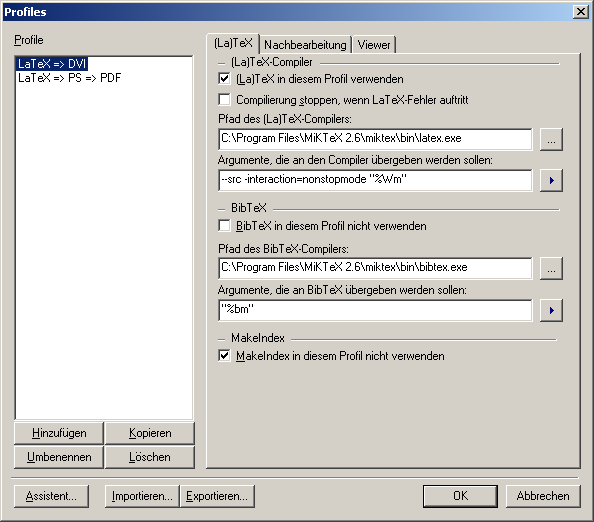
\includegraphics[width=0.49\textwidth]{techniccenter-profile-dvi-26} &
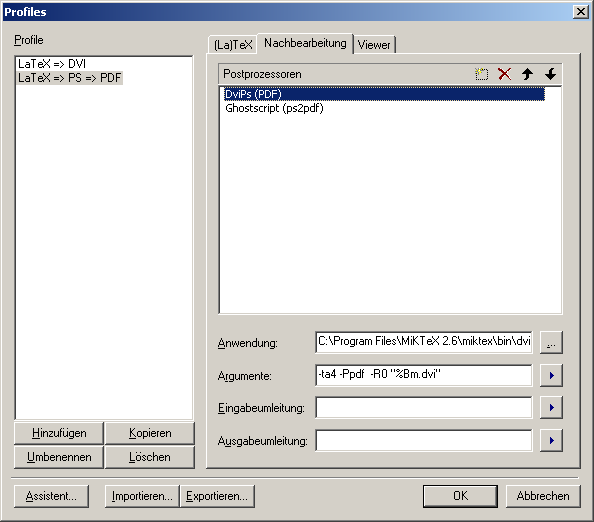
\includegraphics[width=0.49\textwidth]{techniccenter-profile-dvips-26} \\[4pt]
(a) & (b)
\end{tabular}
\caption{Spezifikation der Ausgabeprofile in TeXnicCenter.}
\label{fig:techniccenter-profile-latex}
\end{figure}

In der Datei \verb!tc_output_profiles_sumatra.tco! sind  folgende beiden "`maßgeschneiderten"' Ausgabeprofile für TexNicCenter angelegt (Import über \textsf{Build} $\rightarrow$ \textsf{Define Output Profiles ...}):
\begin{itemize}
	\item \verb!LaTeX => PDF (Sumatra)! -- Standard, direkte Erzeugung von PDF,
	\item \verb!LaTeX => PS => PDF (Sumatra)! -- PDF "`klassisch"' via DVI und PS.
\end{itemize}

\subsubsection{Profil "`\texttt{LaTeX => PDF (Sumatra)}"'}

Das ist das mit diesem Setup normalerweise verwendete Standardprofil.

\paragraph{(La)Tex:}
\begin{itemize}
  \item Path to the (La)TeX compiler: \\
        \begin{small} \verb!C:\Program Files (x86)\MiKTeX 2.9\miktex\bin\pdflatex.exe!\end{small}
  \item Command line arguments to pass to the compiler:\\
\begin{small}
   \verb!-synctex=-1 -interaction=nonstopmode "%pm"!
\end{small}
\end{itemize}

\paragraph{Postprocessor:} 
leer, kein Postprocessor notwendig.

\paragraph{Viewer:}
\begin{itemize}
\item Path of executable: \\
\begin{small}
    \verb!C:\Program Files (x86)\SumatraPDF\SumatraPDF.exe ! \\ 
    \verb!-inverse-search "\"C:\Program Files\TeXnicCenter\TEXCNTR.EXE\" !\\
    \verb!/ddecmd \"[goto('%f','%l')]\""!
\end{small}
%
\item View project's output: \\
\begin{small}
    \checkbox\ Command line argument \\\
    Command: \verb!"%bm.pdf"!
\end{small}
%
\item Forward search:\\
\begin{small}
    \checkbox\ DDE command \\\
    Command: \verb![ForwardSearch("%bm.pdf","%Wc",%l,0)]! \\
    Server: \verb!SUMATRA! \\
    Topic: \verb!Control!
\end{small}
\item Close document before running (La)TeX:\\
\begin{small}
    \checkbox\ Do not close
\end{small}
\end{itemize}


\subsubsection{Profil "`\texttt{LaTeX => PS => PDF (Sumatra)}"'}

Profil ausschließlich für den DVI-PS-Workflow (über DVI und PostScript).

\paragraph{(La)Tex:}
\begin{itemize}
  \item Path to the (La)TeX compiler: \\
        \begin{small} \verb!C:\Program Files (x86)\MiKTeX 2.9\miktex\bin\latex.exe!\end{small}
  \item Command line arguments to pass to the compiler:\\
\begin{small}
   \verb!-synctex=-1 -interaction=nonstopmode "%pm"!
\end{small}
\end{itemize}

\paragraph{Postprocessor:}
\begin{itemize}
  \item DviPS (PDF): \\
        \begin{small} 
        Executable: \verb!C:\Program Files (x86)\MiKTeX 2.9\miktex\bin\dvips.exe! \\
        Arguments: \verb!-ta4 -P pdf -R0 "%Bm.dvi"!
        \end{small}
  \item Ghostscript (ps2pdf):\\
  		\begin{small} 
        Executable: \verb!C:\Program Files (x86)\gs\gs9.04\bin\gswin32c.exe! \\
        Arguments: \verb!-q -dPDFSETTINGS=/prepress -sPAPERSIZE=a4 -dSAFER! \\
         \verb!-dBATCH -dNOPAUSE -sDEVICE=pdfwrite -sOutputFile="%bm.pdf"! \\
         \verb!-c save pop -f "%bm.ps"!
      \end{small}
\end{itemize}

\paragraph{Viewer:}
wie in Profil A. (\texttt{LaTeX => PDF (Sumatra)}).

\section{Tipps und offene Probleme:}

\begin{itemize}
\item \texttt{psfrag} funktioniert nicht mit \texttt{pdflatex} und es gibt auch leider keine Ersatzlösung. 
Wenn man \texttt{psfrag} braucht, dann muss man weiterhin über PostScript 
(\verb!LaTeX => PS => PDF!) arbeiten (was allerdings nunmehr auch mit \texttt{hyperref} kein Problem mehr ist).
%
\item Bei Verwendung des TexWorks-Editors (wird mit MikTeX ausgeliefert) sollte man die Standard-Zeichenkodierung von \emph{Unicode} (utf8) auf \emph{Latin-1} (ISO 8859-1) umstellen.
%
\item Adobe Illustrator kann beim Speichern als PDF die Bounding Box nicht setzen. 
Eine Möglichkeit ist, die Grafik zuerst als EPS zu exportieren und dann mit Acrobat in ein PDF zu konvertieren. 
%
\end{itemize}
\end{comment}



\begin{comment}
\section{Einstellungen für YAP (DVI-Viewer) im DVI-PS-Workflow}
\label{sec:YapEinstellung}

Im Standard-DVI-Viewer YAP lässt sich durch Mausklick auf das DVI-Dokument sehr leicht die zugehörige Stelle im Quelltext finden. Im Normalfall öffnet dann TeXnicCenter das zugehörige \latex-Dokument automatisch an der richtigen Stelle.
Das zugehörige "`Inverse DVI Search"' Kommando sollte sich bereits bei der Installation richtig einstellen.

Falls dies \emph{nicht} funktioniert, kann man in YAP diese Einstellung auch manuell über das Menü \textsf{View}\thinspace$\rightarrow$\thinspace\textsf{Options...} vornehmen, wie in Abb.\ \ref{fig:yap-inverse-search} gezeigt.
In diesem Fall lautet die vollständige Anweisung in "`Command Line"' folgendermaßen:
\begin{center}\footnotesize
\verb!"C:\Program Files (x86)\TeXnicCenter\TEXCNTR.EXE" /ddecmd "[goto('%f', '%l')]"!
\end{center}


\begin{figure}
\centering\small
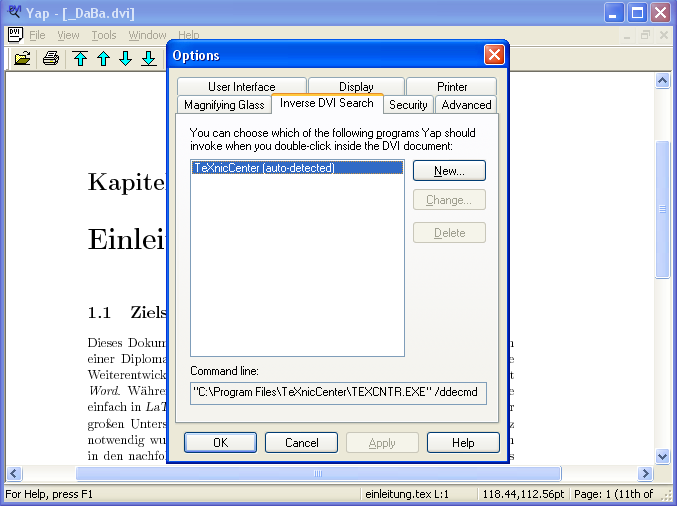
\includegraphics[width=1.0\textwidth]{yap-inverse-search-settings}
\caption{"`Inverse DVI Search"' Einstellung in YAP (über das Menü \textsf{View}\thinspace$\rightarrow$\thinspace\textsf{Options...}).}
\label{fig:yap-inverse-search}
\end{figure}

Latex
C:\Program Files\MiKTeX 2.6\miktex\bin\latex.exe
--src -interaction=nonstopmode "%Wm"

Bibtex
C:\Program Files\MiKTeX 2.6\miktex\bin\bibtex.exe
"%bm"

---

DviPs (PDF)
C:\Program Files\MiKTeX 2.6\miktex\bin\dvips.exe
-ta4 -Ppdf  -R0 "%Bm.dvi"

Ghostscript (ps2pdf)
C:\Program Files\gs\gs8.61\bin\gswin32c.exe
-sPAPERSIZE=a4 -dSAFER -dBATCH -dNOPAUSE -sDEVICE=pdfwrite -dPDFSETTINGS=/prepress -sOutputFile="%bm.pdf" -c save pop -f "%bm.ps"


YAP 
Options -> Inverse Search
"C:\Program Files\TeXnicCenter\TEXCNTR.EXE" /ddecmd "[goto('%f', '%l')]"

\end{comment}

	% Technische Ergänzungen
%\chapter{Inhalt der CD-ROM/DVD}
\label{app:cdrom}

\paragraph{Format:} 
		CD-ROM, Single Layer, ISO9660-Format%
\footnote{Verwenden Sie möglichst ein Standardformat, bei DVDs natürlich
eine entsprechende andere Spezifikation.}


\section{PDF-Dateien}
\begin{FileList}{/}
%\fitem{_DaBa.dvi} Gesamtdokument (DVI-File, ohne Grafiken)
\fitem{_DaBa.pdf} Diplom- oder Bachelorarbeit mit Instruktionen (Gesamtdokument)
\fitem{_PrBericht.pdf} Praktikumsbericht (verkürzte Version der Bachelorarbeit) %
\end{FileList}


\section{\latex-Dateien}

\textbf{Achtung:} Die folgende Auflistung soll nur den Gebrauch dieser Vorlage erleichtern. Es ist bei einer Diplom- oder Bachelorarbeit \ia\ \emph{nicht} notwendig, die zugehörigen \latex-Dateien aufzulisten (wohl aber projektbezogene Dateien, Ergebnisse, Bilder, Kopien von Online-Literatur etc.)!

\begin{FileList}{/}
\fitem{_DaBa.tex} Diplom-/Bachelorarbeit (Hauptdokument) %
\fitem{_PrBericht.tex} Praktikumsbericht (verkürzte Version der Bachelorarbeit) %
\fitem{vorwort.tex} Vorwort %
\fitem{kurzfassung.tex} Kurzfassung %
\fitem{abstract.tex} Abstract %
\fitem{einleitung.tex} Kapitel 1 %
\fitem{diplomschrift.tex} Kapitel 2 %
\fitem{latex.tex} Kapitel 3
\fitem{abbildungen.tex} Kapitel 4 %
\fitem{formeln.tex} Kapitel 5 %
\fitem{literatur.tex} Kapitel 6 %
\fitem{drucken.tex} Kapitel 7 %
\fitem{word.tex} Kapitel 8 %
\fitem{schluss.tex} Kapitel 9 %
\fitem{anhang_a.tex} Anhang A (Source Code) %
\fitem{anhang_b.tex} Anhang B (Inhalt CD-ROM) %
\fitem{anhang_c.tex} Anhang C (Liste der Änderungen) %
\fitem{anhang_d.tex} Anhang D (LaTeX-Quellcode) %
\fitem{messbox.tex} Messbox zur Druckkontrolle %
\fitem{literatur.bib} Literatur-Datenbank (BibTeX-File)
\end{FileList}

\section{Style/Class-Dateien}

\begin{FileList}{/}
\fitem{hgbthesis.cls} LaTeX Class-Datei für Master- und Bachelorarbeiten
\fitem{hgbtermreport.cls} LaTeX Class-Datei für Semesterberichte
\fitem{hgb.sty} LaTeX Style-Datei für alle Hagenberg-Dokumente
\end{FileList}


\section{Sonstiges}

\begin{FileList}{/images}
\fitem{*.ai} Original Adobe Illustrator-Dateien %
\fitem{*.fh11} Original Macromedia Freehand-Dateien %
\fitem{*.jpg, *.png} Original Rasterbilder %
%\fitem{*.eps} Bilder und Grafiken im EPS-Format%
%\fitem{fonts-bakoma/} BaKoMa TrueType Fonts %
\end{FileList}
	% Inhalt der CD-ROM/DVD
%\chapter{Chronologische Liste der Änderungen}


\begin{sloppypar}
\begin{description}
%
\item[2002/01/07]
\verb!\newfloat{program}! repariert (auch ohne Chapter). Dank an Werner Bailer!
%
\item[2002/03/06]
Copyright-Notice an internat.\ Standard angepasst. Dank an Karin Kosina!
%
\item[2002/07/28]
"`Studiengang"' $\rightarrow$ "`Diplomstudiengang"'
%
\item[2003/08/24]
Neues Macro: \verb!\Messbox{breite}{hoehe}! -- zur Kontrolle der 
Druckgröße ohne PS-Datei. Erweiterungen für Bakkalaureatsarbeiten
%
\item[2005/04/09]
Diverse Korrekturen: Captions von Tabellen nach oben gesetzt. 
\texttt{caption} auf neue Versionen adaptiert.
\texttt{subfigure} wird nicht mehr verwendet
%
\item[2006/01/20]
Adaptiert zur Verwendung als Praktikumsbericht 
(2.\ Bakk.-Arbeit)
%
\item[2006/03/24]
Fehler in \verb!\erklaerung! beseitigt (Dank an David Schwingenschlögl)
%
\item[2006/04/06]
Verwendung von T1-Fontencoding zur besseren Silbentrennung bei 
Umlauten etc.
%
\item[2006/06/21]
Neu: Bachelorstudiengang / Masterstudiengang.
Literaturverweise auf Bakk-Arbeiten.
\texttt{upquote.sty} eliminiert (Problem mit TS1-Kodierung).
Verwende Komma (statt Punkt) als Trennzeichen in Dezimalzahlen.
%
\item[2006/09/14]
Anmerkungen zum Thema Plagiarismus.
%
\item[2007/07/16]
Ergänzungen für Code-Listings (listings) und Algorithmen 
(\texttt{algorithmicx}).
BiBTeX-Datei aufgeräumt, Verwendung der Literaturformate 
verbessert.
Komma (statt Punkt) als Trennzeichen in Dezimalzahlen wieder 
entfernt.
Verwendung der \texttt{ae}-Fonts eliminiert (\texttt{cm-super} Fonts müssen 
installiert sein, ab MikTeX 2.5). 
Beispiel für Ersetzung in EPS-Dateien mit \texttt{psfrag}.
%
\item[2007/10/04]
Version 5.90: Das Laden der Pakete \verb!inputenc! (Option \texttt{latin}) und 
\verb!graphicx! (Option \texttt{dvips})
aus der Hauptdatei in die \texttt{sty}-Datei übertragen; \texttt{upquote} funktioniert nun.
Paket \texttt{eurosym} ergänzt für Euro-Symbol (Anregung von Andreas 
Doubrava).
Problem mit \texttt{color}-package repariert (gerasterter PDF-Ausdruck).
Hinweise bzgl.\ Literatur ergänzt (\texttt{month}, \texttt{edition}),
BibTeX-Datei gesäubert.
Hinweis zum Einfügen von vertikalem Abstand zwischen Absätzen.
Mathematik aufgeräumt, Verwendung von \texttt{amsmath}, 
Fallunterscheidungen.
Diverse Änderungen bei Tabellen und Programmkode.
Beispiele für BibTeX-Angaben von Spezialquellen: Audio-CDs, 
Videos, Filme. Einbinden von Dateien mit \verb!\include{..}!
Neue Datei: \verb!_SimpleReport.tex! für kurze Reports (Projekte etc.).
%
\item[2007/11/11]
Version 5.91: Hinweise zur Einstellung der Output-Profile in
TexNicCenter, Inverse Search Einstellung in YAP im Anhang.
%
\item[2008/04/01]
Version 6.00beta -- kompletter Umbau!
Auslagerung der Doku\-menten-relevanten Teile in eine eigene 
\emph{class}-Datei (\texttt{hgbthesis.cls}) mit Optionen.
Die neue Style-Datei \texttt{hgb.sty} ist nun unabhängig vom 
Dokumententyp und nicht mehr kompatibel mit älteren Versionen!
Die Liste der Änderungen ist jetzt in der Datei \verb!_ChangeLog.tex!
(DIESE Datei) und diese wird im Anhang eingebunden.
Heading-Style auf Sans Serif geändert (ohne grausliche "`Caps"').
%
\item[2008/05/22]
Neue Vorlage für Technical Reports (Klasse \texttt{hgbreport.cls}).
Spracheinstellung nunmehr mit \texttt{babel}-Paket, Hauptsprache
des Dokuments kann als Option der Klasse angegeben werden.
Sprachumschaltung innerhalb des Dokuments funktioniert nun
richtig. Mit der Sprachoption \texttt{german} wird automatisch die neue deutsche 
Orthographie (\texttt{ngerman}) verwendet.
\texttt{babelbib} wird zur Formatierung des Literaturverzeichnisses
verwendet (neue BibTeX-Style-Optionen!).
Header werden nunmehr mit \texttt{fancyhdr}-Paket erzeugt.
Versionsnummerierung von \texttt{.cls} und \texttt{.sty} Files wird beendet 
(ab jetzt gilt: \emph{Datum} = \emph{Version}). 
%
\item[2008/06/10]
Neues Listing-Environment \texttt{PhpCode}; bei allen Listing-Eviron\-ments ist nun 
\texttt{mathescape=false} (kein Math-Mode nach \verb!$!). 
Bug bei Sprachumschaltung auf \texttt{ngerman} beseitigt.
%
\item[2008/08/15]
Diverse Kleinigkeiten in Literaturangaben überarbeitet (Dank an Norbert Wenzel), Spracheinstellung vereinheitlicht, Umlaute in \texttt{.bib}-Datei ersetzt.
%
\item[2008/10/15] 
Zusätzliche Hinweise zur MikTeX-Installation (Windows) sowie LaTeX unter Mac OS~X und Linux.
Liste der Abkürzungen ergänzt.%
\item[2008/11/15] 
Diverse Schreibfehler korrigiert (Dank an Silvia Fuchshuber). Hinweis auf 
\texttt{sloppypar}-Umgebung.
%
\item[2008/12/09] 
BibTeX-Tools: neuer Hinweis auf JabRef ergänzt, BibEdit entfernt (ist nicht mehr auffindbar).
%
\item[2009/02/09]
\texttt{hgb.sty}: Option "`\texttt{spaces}"' zu \texttt{url}-Package ergänzt (ermöglicht gezielten Zeilenumbruch in URLs). 
Im allgemeinen Setup für \texttt{listings}: \texttt{keepspaces=true};
Obsoletes Environment \texttt{sourcecode} deaktiviert.
Escape-Mode für \texttt{LaTeXCode}-Umgebung geändert.
\verb!_DaBa.tex!: Hinweis auf die Verwendung von \verb!\urldef! für die Angabe von URLs in Captions. \texttt{diplom} (statt \texttt{master}) als Standard-Dokumententyp in \verb!_DaBa.tex! ("`Diplomarbeit"'). Neuer Abschnitt zum Umgang mit ``Quellenangaben in Captions''.
\texttt{literatur.bib}: alle URLs (bisher in \texttt{note}-Einträgen) auf \verb!url={..}! geändert.
%
\item[2009/04/14]
Hinweis zum Einfügen einfacher Anführungszeichen ergänzt.
%
\item[2009/07/18]
Literaturangaben korrigiert und ergänzt.
%
\item[2009/11/27]
Experimentelle Version: Massive Änderungen, Umstieg auf \texttt{pdflatex}.
%
\item[2010/06/15]
Erstes Release der neuen Version mit \texttt{pdflatex}.
\item[2010/06/23]
Konflikt zwischen \texttt{pdfsync}-Package und \texttt{array}-Package (wird relativ häufig benutzt) durch \verb!\RequirePackage[novbox]{pdfsync}! behoben.
Seitenunterkante durch \verb!\flushbottom! fixiert,
variablen Absatzzwischenraum reduziert.
\item[2010/07/27]
Sprache der Erklärungsseite auf "`\texttt{german}"' fixiert (auch wenn die Hauptsprache des Dokuments  Englisch ist). %Datumsproblem - Hinweis von Philipp Winter
\item[2010/12/03]
Anmerkungen und Beispiele zum Zitieren von Gesetzestexten und Videos (Zeitangabe) ergänzt.
Hinweis auf \verb!\nolinkurl{..}! zur Angabe von Dateinamen.
\item[2011/01/29]
Einbau der Creative Commons Lizenz und entsprechender Hinweis in 
Abschnitt \ref{sec:HagenbergEinstellungen}. Neue Makros
\verb!\strictlicense!,
\verb!\cclicense! und
\verb!\license{...}!.
BibTeX-Einträge für Audio-CDs und Filme korrigiert, Beispiel für Online-Video ergänzt.
\item[2011/02/01]
Neues Makro \verb!\betreuerin{..}! zur Angabe einer (weiblichen) Betreuerin. 
%
\item[2011/06/26]
Umstellung der gesamten Literaturverwaltung auf \texttt{biblatex} mit dem Ziel, 
getrennte Abschnitte für verschiedene Kategorien von Einträgen im Quellenverzeichnis
zu ermöglichen. Die Wahl fiel auf \texttt{biblatex} (es gäbe andere Optionen), weil
damit BibTeX weiterhin nur einmal aufgerufen werden muss (und nicht für
mehrere Dateien). Damit verbunden sind allerdings massive Änderungen bei der
Syntax der BibTeX-Felder und es gibt auch mehrere neue Felder.
Aktuell sind 3 Kategorien von Quellen vorgesehen, entsprechende Änderungen in 
\nolinkurl{hgbthesis.cls}. Der klassische BibTeX-Workflow wird aktuell nicht
mehr unterstützt, die Möglichkeit einer künftigen Dok-Option ist aber 
vorgesehen. Das Literatur-Kapitel ist komplett überarbeitet, die .bib-Datei
wurde ausgemistet. Neu ist die Empfehlung zur Aufnahme von Bildquellen
in das Quellenverzeichnis, womit lange URLs in Captions (dort sind keine
Fußnoten möglich) nicht mehr notwendig sind. 
"`Persönliche Kommunikation"' als Literaturquelle entfernt (den Inhalt
von Interviews sollte man direkt im Anhang wiedergeben).
Das verwendete Bildmaterial wurde
erneuert, aktuell werden nur mehr Public Domain Bilder verwendet. 
Das Kapitel "`Hinweise für Word-Benutzer"' wurde endgültig entfernt.
\verb!\flushbottom! wieder auf \verb!\raggedbottom! geändert, um übermäßige 
Abstände zwischen Absätzen zu vermeiden.
%
\item[2012/05/10]
Hinweis auf die in Österreich bislang nicht zulässige Verwendung von "`Masterarbeit"'
entfernt, \texttt{master} ist nunmehr die Default-Dokumentenoption.
Anmerkungen zu lästigen \texttt{biblatex}-Warnungen ergänzt.
Angaben für Windows-Programmpfade auf Win7 angepasst, 
MikTeX 2.9 als Minimalerfordernis.\newline
Überflüssige Makros \verb!\damonat! und \verb!\dajahr! endgültig entfernt, statt
\verb!\abgabemonat! und \verb!\abgabejahr! ist nun das neue Makro
\verb!\abgabedatum{yyyy}{mm}{dd}! vorgesehen (unter Verwendung von internen Zählern).
Zur Formatierung von Datumsangaben wir das \texttt{datetime}-Paket verwendet.
\newline
Neue Fassung der eidesstattlichen Erklärung (inkl.\ englischer Version).\newline
PDF-Suche auf \texttt{synctex} umgestellt (\texttt{pdfsync}-Paket ist veraltet und
wird nun nicht mehr verwendet).
\newline
Die älteren Dateiversionen von \texttt{algorithmicx.sty} und \texttt{alg\-pseudo\-code.sty}
(bisher explizit beigefügt) wurden weggelassen.
\newline
Hinweis auf die \emph{Latin Modern Roman} OTF-Schriften ergänzt.
%
\item[2012/07/21]
Quellenverzeichnis: sprachabhängige Einstellung der Überschriften eingerichtet.
Titel des Quellenverzeichnisses auf "`Quellenverzeichnis"' (DE) \bzw\ "`References"' (EN) 
fixiert. Makro \verb!\MakeBibliography! hat damit keinen erforderlichen Parameter mehr.
%
\item[2012/09/17]
Wegen Änderungen im \texttt{biblatex}-package (Version 1.7, 2011/11/13) die Verwendung von
BibTeX als backend eingestellt (\texttt{backend=bibtex8}).
%
\item[2012/10/13]
Option \texttt{lowtilde} beim URL-package eingestellt (erzeugt \url{~} statt \verb!~!).
%
\item[2012/12/01]
In Abschnitt \ref{sec:FormatierungVonProgrammcode} zusätzliche Code-Umgebungen ergänzt:
\texttt{JsCode},
\texttt{PhpCode},
\texttt{HtmlCode},
\texttt{CssCode},
\texttt{XmlCode}.
%
\item[2012/12/08]
Die Code-Umgebungen in Abschn.\ \ref{sec:FormatierungVonProgrammcode} ergänzt und 
zur Verwendung von optionalen Argumenten erweitert (Hinweise in Abschnitt 
\ref{sec:FormatierungVonProgrammcode} auf die Argumente
\texttt{firstnumber=last} und \texttt{numbers=none}).
Quellenverzeichnis: den Eintragstyp \texttt{@software} für Games empfohlen und im Verzeichnis
der Kategorie \emph{avmedia} zugeordnet (Tab.~\ref{tab:BibKategorien} ergänzt). 
Game-Beispiel (von Manuel Wieser) und zusätzliche Tabelle \ref{tab:QuellenUndEintragstypen}
zur besseren Übersicht eingefügt.
%
\item[2013/05/17]
Wichtigste Änderung ist die vollständige Umstellung auf \textbf{UTF-8} unter Beibehaltung des 
\texttt{pdflatex}-Workflows. 
Damit sind zahlreiche weitere Modifikationen verbunden:
\newline
Alle Dateien (auch \texttt{.cls}, \texttt{.sty} und \texttt{.bib}) wurden auf UTF-8 konvertiert.
Damit sollte es auch keine Probleme mehr mit Umlauten und Sonderzeichen unter MacOS geben.
\newline
Die verwendete Standard-Schriftfamilie ist nun "`Latin Modern"' (\texttt{lmodern}). 
Sie ersetzt die "`CM-Super"' Schriften, mit denen es immer wieder Installationsprobleme gab.
Weiters wird jetzt das \texttt{cmap}-Paket zur besseren Such- und Kopierbarkeit von PDFs verwendet.
\newline
Das \texttt{listings}-Paket wurde durch \texttt{listingsutf8} ersetzt und für Umlaute im Quellcode adaptiert.
Eventuell sind weitere Adaptierungen notwendig.
\newline
\texttt{biber} (min.\ Version 1.5!) wird nun anstatt \texttt{bibtex} (unterstützt keine UTF-8 Dateien) verwendet,
zusammen mit \texttt{biblatex} (Version 2.5).
Die Anweisung \verb!\bibliography! wird (wieder) verwendet, allerdings nun in der Präambel,
um die \texttt{.bib}-Datei im Fileverzeichnis anzuzeigen.
\newline
Das Makro \verb!\C! (für die Menge der komplexen Zahlen \Cpx) musste wegen Problemen in der T1-Kodierung
ersetzt werden und heißt nun \verb!\Cpx!. Die Makros 
\verb!\R!, \verb!\Z!, \verb!\N!, \verb!\Q! und \verb!\Cpx! können nun auch außerhalb des Mathematik-Modus verwendet werden.
\newline
Der DVI-PS-PDF Workflow wird ab dieser Version überhaupt nicht mehr unterstützt. 
Damit ist auch das \texttt{psfrag}-Paket nicht mehr verwendbar. Entspechende Hinweise 
wurden aus dem Text entfernt.
\newline
\texttt{hyperref} wurde auf UTF-8 umgestellt.
Die grässlichen Standard-Rahmen und Farben der automatischen \texttt{hyperref}-Links wurden entfernt \bzw\ durch 
dezentere Farben ersetzt. Dadurch wird auch die Screen-Version der PDFs wieder lesbar.
\newline
Im Quellenverzeichnis wurde versuchsweise die \texttt{backref}-Option aktiviert. 
Damit werden bei allen Einträgen auch die zugehörigen Zitierstellen angegeben
(erscheint durchaus sinnvoll).
\newline
Die bisherigen Korrekturen zur \texttt{biblatex}-Formatierung wurden entfernt, 
alles arbeitet nun mit Standard-Einstellungen. Die ursächlichen Probleme in \texttt{biblatex}
scheinen in der aktuellen Version behoben zu sein.
\newline
Das Output-Profil für TeXnicCenter wurde für den neuen Workflow mit \texttt{biber} adaptiert und liegt nun in
\nolinkurl{_tc_output_profile_sumatra_utf8.tco}.
\newline
Das Windows-Script \verb!_clean.bat! wurde entfernt, da TeXnicCenter nun ein eigenes "`Clean Project"'-Kommando aufweist (in "`Build"').
\newline
Allgemeine Einstellungen zu \emph{headings} und \emph{biblatex} wurden aus der Datei \texttt{hgbthesis.cls} entfernt und in 
\texttt{hgbheadings.sty} \bzw\ \texttt{hgbbib.sty} verlagert. Diese können nun unabhängig verwendet werden (s.\ Beispiel in 
\texttt{\_TermReport.tex}).
\newline
Die Klassen-Datei \texttt{hgbtermreport.cls} wurde eliminiert, das Dokument \texttt{\_TermReport.tex} basiert nunmehr
auf der generischen LaTeX-Klasse \texttt{report}  und verwendet keine eigene \texttt{.cls} Datei mehr.
%
\item[2014/11/05]
Neu: Logo auf der Frontseite bei allen Dokumententypen. Dazu gibt es ein neues Kommando
\verb!\logofile{pic}!, wobei \verb!pic! der Name eine PDF-Datei im
Verzeichnis \verb!images/! ist. Falls \emph{kein} Logo erwünscht ist, 
kann man die Zeile einfach weglassen oder durch \verb!\logofile{}! ersetzen.
\newline
\texttt{hyperref}-Einstellungen: Einfärbung der Links wieder entfernt (\texttt{colorlinks = false}), weil beim Druck
nicht abschaltbar. Stattdessen einheitliche (dezente) Rahmen für alle Linkarten.
Zahlreiche Tippfehler eliminiert (Dank an Daniel Karzel).
\newline
Wegen eines Bugs in \texttt{biblatex 1.9} wurden die expliziten Abteilungen (\verb!\-!) in \texttt{literatur.bib}
vorübergehend entfernt (mit entsprechenden Folgen im Ergebnis). Der Bug soll in \texttt{biblatex 2.0} (derzeit noch
nicht verfügbar) behoben sein.
\newline
Package \texttt{color} auf \texttt{xcolor} geändert. In \texttt{hgb.sty} neues "`Convenience-Makro"' \verb!\etc! ergänzt.
Output-Profil für TeXnicCenter/SumatraPDF (Windows) repariert, forward/inverse Search funktioniert nun
(Datei \verb!_tc_output_profile_sumatra_utf8.tco!).
%
\item[2015/04/28]
Paket \texttt{subdepth} (zur verbesserten Platzierung von Sub- und Superscripts) 
in hgb.sty ergänzt.
%
\item[2015/07/14]
Hinweis und Abhilfe für die (nicht automatische) Silbentrennung in zusammengesetzten Wörtern.
Neu in \texttt{hgbheadings.sty}: \verb!\RequirePackage[raggedright]{titlesec}! verhindert Blocksatz
in Section-Überschriften (sehr unschön bei längeren Überschriften). 
Neu (in Abschn.~\ref{sec:GraphicOverlays}): Beispiel für die Verwendung des \texttt{overpic}-Pakets
zur Annotierung von importierten Grafiken (verwendet zudem das \texttt{pict2e}-Paket).
%
\item[2015/08/03]
Logo-Datei auf \texttt{logo.pdf} umbenannt.
\item[2015/09/17]
Anweisung \verb!\RequirePackage[utf8]{inputenc}! in die Doku\-menten\-dateien (\texttt{\_xxx.tex})
verschoben (auf Anregung von Markus Kohm: "`\ldots für die Verwendung von lualatex oder xelatex 
ist die Anweisung in hgb.sty störend, da bei diesen beiden aufgrund der nativen utf8-Unterstützung 
\texttt{inputenc} keinesfalls verwendet werden darf"').
\item[2015/09/19]
\texttt{hgb.sty} aufgeräumt.
Makros \verb!\@savesymbol! und \verb!\@restoresymbol! aus \texttt{hgb.sty} entfernt
(wurden nicht mehr verwendet; ggfs.\ Paket \texttt{savesym} als Ersatz).
Makro \verb!\optbreaknh! (optional break with no hyphen) auf \verb!\obnh! umbenannt.
Teile von \texttt{hgb.sty} in neue Dateien \texttt{hgbabbrev.sty} (div.\ Abkürzungen)
und \texttt{hgblistings.sty} (Code-Listings) verschoben.
Hintergrundtönung der Code-Listings heller (auf 5\% Grau) eingestellt.
Layout: \verb!\textfraction! auf 0.1 (statt fehlhafterweise 0.01) eingestellt.
\texttt{hgbbib.sty}: \verb!\clearpage! am Beginn des Quellenverzeichnisses entfernt
(für \texttt{article}-Template).
\item[2015/09/19]
Alle \texttt{.cls} und \texttt{.sty} Dateien sind jetzt ANSI-codiert (Header eingefügt), wie
laut CTAN-Richtlinien vorgesehen. Umlautzeichen wurden durch Makros ersetzt.
Nur \texttt{hgblistings.sty} ist weiterhin UTF-8 (wegen notwendiger literaler Umlaute).
\verb!\RequirePackage[utf8]{inputenc}! steht sonst nur mehr am Beginn
der jeweiligen (\texttt{.tex}) Haupttextdatei.
\item[2015/10/29]
Verwendung von "`In:"' im Quellenverzeichnis vor \texttt{article}-Einträgen
(Eigenart von biblatex) durch passendes Makro in \texttt{hgbbib.sty} unterbunden 
(Dank an S.\ Dreiseitl).
\item[2015/11/04]
Hinweise in Abschnitt \ref{sec:Software} auf TeXstudio unter Windows, Mac OS und Linux.
Release-Ausgabe.
\end{description}

\end{sloppypar}




%\section*{To Do} 
%\begin{itemize}
%\item Inkscape
%\item biblatex Bib-Driver für audio, video etc. ergänzen.
%\item Mathematik umbauen, typische Fehler stärker berücksichtigen (ua. Leerzeilen vor/nach Gleichungen).
%\item Literaturempfehlungen zum Schreiben von Diplomarbeiten
%\item Hinweise für Literatursuche (Bibliotheksverbund, CiteSeer,...)
%\end{itemize}





	% Chronologische Liste der Änderungen
%\chapter{\latex-Quellkode}
\label{app:latex}

\section*{Hauptdatei {\tt\_DaBa.tex}}

\begin{footnotesize}
\verbatiminput{_DaBa.tex}
\end{footnotesize}


%\vspace*{2cm}
\hrule
\hrule

\paragraph{Anmerkung:}
Das sollte nur ein \emph{Beispiel} für die Einbindung von Quellcode
in einem Anhang sein. Der \latex-Quellkode der eigenen
Diplomarbeit ist meist \emph{nicht} interessant genug, um ihn hier
wiederzugeben!

	% Quelltext dieses Dokuments

%%%----------------------------------------------------------
%\MakeBibliography
%%%----------------------------------------------------------

%%%Messbox zur Druckkontrolle
%\chapter*{Messbox zur Druckkontrolle}



\begin{center}
{\Large --- Druckgröße kontrollieren! ---}

\bigskip

\Messbox{100}{50} % Angabe der Breite/Hoehe in mm

\bigskip

{\Large --- Diese Seite nach dem Druck entfernen! ---}

\end{center}



\end{document}
